\documentclass[a4paper,12pt,oneside,openright]{book}

\usepackage[italian]{babel}
%\usepackage[pdfencoding=auto,psdextra]{hyperref}
\usepackage[T1]{fontenc}
\usepackage[utf8]{inputenc}
\usepackage[usenames,dvipsnames,svgnames,table]{xcolor}
\usepackage{amsmath}
\usepackage{amsthm}
\usepackage{amssymb}
\usepackage[pdfencoding=auto,psdextra]{hyperref}
\usepackage{color}
\usepackage{fancyhdr}
\usepackage{float}
\usepackage{graphicx}
\usepackage{latexsym}
\usepackage{listings}
\usepackage{lmodern}
\usepackage{setspace}
\usepackage{verbatim}
\usepackage{biblatex}

% C++
%\newcommand*{\Cpp}{{\textrm{C}\nolinebreak[4]\hspace{-.05em}\raisebox{.4ex}
%{\tiny\bf ++}}}

% SQLite
%\newcommand*{\sqlite}{{\textrm{SQLite}}}


\begin{document}

\lstset{
  basicstyle=\ttfamily\footnotesize,
  breaklines=true,
  frame=single,
  keepspaces=true,
  numbers=left
}

\begin{titlepage}
  \hypersetup{pageanchor=false}

  \begin{center}
    \medskip

    \begin{figure}
      \centering
      
\includegraphics[scale=0.52]{logouni.png}
    \end{figure}

    %\begin{LARGE}
     % UNIVERSIT\`A DEGLI STUDI DI PARMA \\
      %\medskip
    %\end{LARGE}

    \begin{Large}
      Dipartimento di Matematica e Informatica \\
      \medskip
      Corso di Laurea in Informatica \\
      \medskip
      \underline{Tesi di Laurea} \\
      \vspace{2.0cm}
      
      \begin{huge}
        \textbf{Progettazione e sviluppo di un sistema cloud di monitoraggio di smart objects su reti eterogenee} \\
      \end{huge}
      
      \vspace{2.0cm}
      
      
		  \begin{flushleft}
		    Candidato: \\
		    \textbf{Francesco Salvatore} \\
		  \end{flushleft}
	  \vspace{1.0cm}
	  
	  \begin{minipage}{.45\linewidth}
		  \begin{flushleft}
		    {\small Relatore:} \\
		    \textbf{\small{Prof. Roberto Alfieri}}
		  \end{flushleft}
	  \end{minipage}
	  \hfill
	  \begin{minipage}{.45\linewidth}
		  \begin{flushright}
		    {\small Correlatore:} \\
		    \textbf{\small{Prof. Laura Belli}}
		  \end{flushright}
	   \end{minipage}
      
      \vspace{2.0cm}
      
      Anno Accademico 2014/2015
    \end{Large}

  \end{center}

\end{titlepage}


\tableofcontents

\pagestyle{empty}

\begin{flushright} 
  \emph{Alla mia famiglia e ad Ilaria, \\ che mi hanno sempre sostenuto.}
\end{flushright}

\pagestyle{fancy}
\renewcommand{\chaptermark}[1]{\markboth{#1}{}}
\renewcommand{\sectionmark}[1]{\markright{#1}{}}
\fancyhf{}
\rhead{\rightmark}
\cfoot{\thepage}

\phantomsection
\addcontentsline{toc}{chapter}{Introduzione}
\chapter*{Introduzione\markboth{}{Introduzione}}

Siamo sempre più circondati dalla tecnologia, che ha oramai pervaso quasi ogni aspetto della nostra vita. Sempre più utilizziamo strumenti elettronici che hanno il compito di rendere la qualità della nostra vita migliore e sempre più lo sviluppo tecnologico ha portato alla riduzione in termini di dimensioni di oggetti un tempo ingombranti e poco maneggevoli. Oggi è normale, per esempio, salire in macchina e connettere il proprio smartphone al sistema di entertainment del veicolo per ascoltare musica o utilizzare il navigatore, oppure archiviare migliaia di documenti in oggetti poco più grandi di una moneta, o ancora indossare orologi in grado di registrare e monitorare i nostri parametri vitali.

Parallelamente alla miniaturizzazione elettronica è maturata un'altra tecnologia che ha invaso il nostro vivere comune: Internet. Il mezzo di comunicazione oggi padrone dello scambio di informazioni è cresciuto esponenzialmente dalla sua nascita negli anni '60, attraversando diverse fasi fino a giungere all'attuale era dell'Internet of Things, l'Internet degli oggetti.
\\\\L'unione delle due cose ha dato vita all'Internet of Things, oggetti interconnessi in grado di raccogliere e scambiare dati tra di loro.
\\\\L'obiettivo è quindi quello di sviluppare un sistema in grado di monitorare questi oggetti e notificare, mediante connettori definiti, i dati raccolti o eventuali cambiamenti di questi. Il sistema deve essere scalabile, data la potenziale mole di oggetti monitorabili, portabile e soprattutto interoperabile, ovvero deve essere in grado di raccogliere informazioni provenienti da fonti architetturalmente differenti.

\chapter{L'Internet of Things}
L'Internet of Things, spesso abbreviato in IoT, è il nuovo paradigma in cui il mondo virtuale è strettamente integrato con il mondo reale. Secondo il \textit{Cluster of European Research Projects on the Internet of Things} (CERP-IoT) può anche essere definito come una infrastruttura di rete globale o locale con capacità di autoconfigurazione basata su protocolli standard ed interoperabili, dove gli oggetti fisici e virtuali hanno un'identità, personalità virtuale e utilizzano interfacce intelligenti, oltre ad essere perfettamente integrati nella rete, appunto, Internet.
\\L'IoT si basa quindi sull'idea di mettere in comunicazione, tramite protocolli standardizzati e ben definiti, oggetti variegati - come sensori, attuatori, microcontrollori, smartphone, PC ma anche elettrodomestici, veicoli, interi edifici ecc - che sono individualmente indirizzabili e perfettamente in grado di interagire tra loro, cooperando a formare una unica rete che ha un preciso scopo.
\\Questi oggetti, che hanno la caratteristica di poter interagire non solo con utenti umani ma anche con altri oggetti, prendono il nome di \textit{smart objects} e di conseguenza le reti formati dagli smart objects saranno denominate \textit{smart networks}.
\\L'IoT può essere vista quindi come una naturale evoluzione delle tecnologie e della rete Internet. Gli oggetti si rendono riconoscibili e sono in grado di trasmettere dati sul loro stato attuale, oltre che acquisirne da altri oggetti, non necessariamente situati in aree geografiche circostanti. Potremmo infatti avere un oggetto a New York che trasmette dati ad un altro oggetto a Roma, e quello di Roma ricevere dati anche da un terzo oggetto situato a Tokio.
\\L'obiettivo dell'IoT è fare si che il mondo virtuale si "fonda" con quello reale, dando una vitalità elettronica alle cose e ai luoghi dell'ambiente fisico.
\\\\Le aspettative di crescita, secondo gli esperti, sono esponenziali. \textit{Gartner}, società leader nella consulenza strategica per l'ICT, stima che nel 2020 saranno circa 26 miliardi gli oggetti connessi alla Rete, secondo \textit{ABI Research} si supereranno i 30 miliardi, mentre \textit{Cisco} parla addirittura di 50 miliardi di smart objects interconnessi. La diffusione accellerata di questi oggetti cambierà radicalmente il nostro modo di vivere, e in maniera più veloce rispetto a quanto abbiano fatto altre tecnologie nel passato, che porta a riflettere sulle conseguenze di questi cambiamenti così repentini, soprattutto in termini di privacy e controllo umano.
\\Peter-Paul Verbeek, professore di filosofia della tecnologia all'Università di Twente, afferma che la tecnologia già oggi ha una forte influenza sulle decisioni morali, che a loro volta influenzano l'agire dell'uomo, la sua privacy e la sua autonomia. Altri, come Justin Brookman, temono che le enormi quantità di dati potenzialmente raccolte da queste reti possano diventare oggetto di marketing, analizzando oltre ogni limite di privacy i comportamenti e le abitudini delle persone.
\\Anche alcune riviste del mondo IT rivolte ai consumatori, come Wired, hanno espresso preoccupazione circa lo sviluppo e la diffusione quasi incontrollata di dispositivi in grado di mappare la vita delle persone in ogni luogo e momento.
\begin{figure}[hb]
\centering
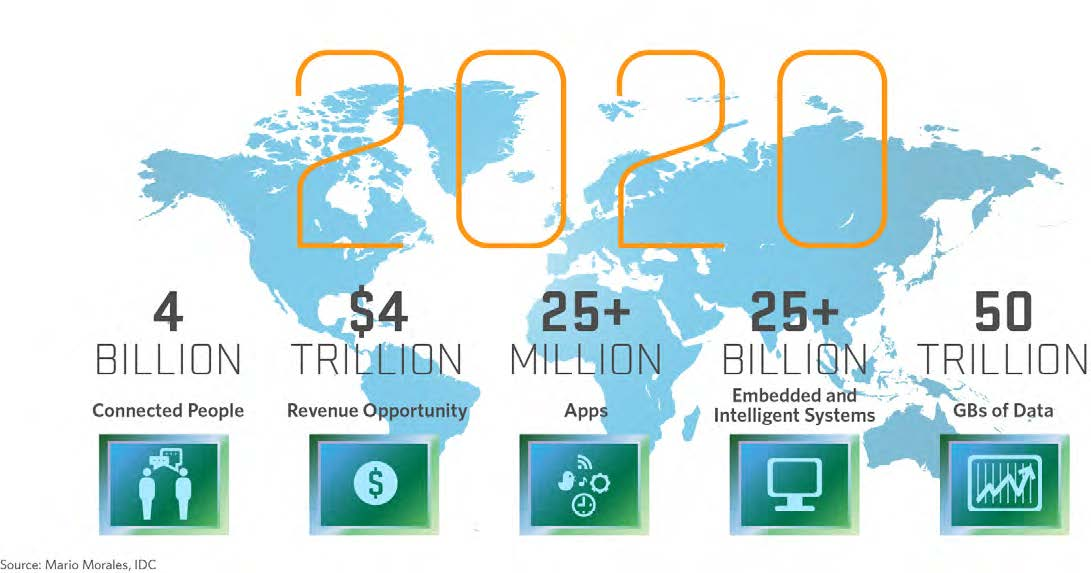
\includegraphics[scale=1.00]{immagini/iot-2020.jpg}
\caption{\textit{Le prospettive per l'IoT nel 2020}}
\end{figure}


\section{Cenni storici}
Il termine IoT viene coniato nel 1999 da Kevin Ashton, direttore esecutivo e co-fondatore dell'\textit{Auto-ID Research Center} al Massachussets Institute of Technology, durante una presentazione per la \textit{Procter \& Gamble}, di una tecnologia RFID (\textit{Radio Frequency Identification}) che avrebbe rivoluzionato e ottimizzato la loro supply chain. Ashton chiamò la sua presentazione "Internet of Things" semplicemente perchè all'epoca Internet era il trend più gettonato e il suo scopo era impressionare la dirigenza dell'azienda.
\\Sebbene dunque il termine sia di stampo recente, le tecnologie, i concetti e la ricerca che sono alla base dell'IoT risalgono anche fino a trent'anni prima.
\\Un contributo importante lo si deve riconoscere sicuramente ad ALOHAnet, sviluppata da Norman Abramson agli inizi degli anni settanta, prima reale sperimentazione di trasmissioni digitali wireless, precursore e apriporta dell'odierno WiFi e di altre tecnologie radio.
\\Un altro importante passo fu sicuramente il brevetto ottenuto nel 1973 dall'italo-americano Mario Cardullo per quello che è considerato a tutti gli effetti il primo prototipo di tag RFID passivo.
\\Nel 1976 \textit{AT\&T} e \textit{MIT} organizzano una conferenza sui possibili sviluppi futuri della tecnologia e il \textit{Bell Systems}, una rivista di notizie riguardanti la tecnologia, ha l'occasione di intervistare l'autore di \textit{2001: Odissea nello spazio}, Arthur C. Clarke, che predice abbastanza accuratamente quale sarà la direzione tecnologica degli anni a venire. Scrive infatti:
\begin{quotation}
Stiamo per avere dispositivi che ci permetteranno di inviare molte più informazioni ai nostri amici. Saranno in grado di vederci, noi saremo in grado di vedere loro, scambieremo grafici, immagini, libri e così via. Il dispositivo di comunicazioni ideale potrebbe essere una televisione ad alta definizione con una tastiera e, attraverso questo, potremo scambiare ogni tipo di informazione. Mandare messaggi agli amici...potranno ricevere messaggi durante la notte e leggerli quando si svegliano. Potremo richiedere al dispositivo tutte le informazioni che vogliamo: dai voli aerei ai prezzi nei supermercati, dai libri che vogliamo leggere alle notizie. La macchina cercherà queste informazioni per noi e ce le restituirà selettivamente, secondo i nostri gusti e le nostre abitudini.
\end{quotation}
\vspace{1.0cm}
Nel 1990 l'Olivetti Research Laboratory di Cambridge sviluppa un sistema di localizzazione indoor basato su badge personali a infrarossi. Si tratta di un primo esperimento di utilizzo di segnali radio per localizzazioni in aree circoscritte. Gli Active Badge, così sono chiamati dal team di sviluppo, erano di dimensioni e peso ridotti e trasmettevano un segnale IR ogni 15 secondi, segnale che veniva captato da apposite stazioni posizionate in punti strategici dell'area da coprire. Fu scelto di utilizzare la banda IR per diverse ragioni: innanzitutto il raggio di copertura del segnale era limitato (circa 6 metri in linea d'aria) il che evitava che la trasmissione fosse captata da più sensori contemporaneamente; il segnale non era in grado di penetrare muri e grossi ostacoli, che rendeva i rilevamenti molto più accurati; e infine, ma non meno importante, i trasmettitori e i ricevitori IR erano di ridotte dimensioni e costavano meno delle tecnologie concorrenti.
\\Il progetto è estremamente interessante da un punto di vista storico dell'Internet of Things in quanto nel documento di presentazione redatto all'epoca vi era una rappresentazione grafica che includeva la possibilità di connettere le reti formate dai trasmettitori/ricevitori ad Ethernet, e di conseguenza alla rete Internet. Si ipotizza infatti la possibilità di inserire dei calcolatori nel mezzo in grado di ottenere i dati "telemetrici" rilevati dai sensori e renderli maggiormente "human-readable". Gli Active Badge inoltre erano in grado, mediante un sensore di luminosità, di capire se erano stati lasciati in ufficio la notte o il fine settimana, disattivando il circuito di trasmissione per risparmiare batteria. Il progetto prevedeva anche l'inserimento di un accellerometro per migliorare ulteriormente il risparmio energetico (l'oggetto trasmette solo se è in movimento), ma tuttavia si dovette desistere dall'integrarlo in favore di dimensioni più ridotte.
\\\\Ma il primo vero oggetto connesso alla rete Internet fu "l'Internet Toaster", sviluppato da John Romkey e Simon Hackett, sempre nel 1990. Il toaster, un grande classico Sunbeam, era in grado, tramite protocollo SNMP-MIB (\textit{Simple Networking Management Protocol - Management Information Base}), di notificare l'avvenuta cottura del toast e di spegnersi automaticamente al raggiungimento di questa. Un anno più tardi la macchina venne perfezionata, aggiungendo la capacità di regolare il grado di tostatura delle fette di pane e di prendere, tramite pinza robotica, la fetta di pane da tostare da un piatto posto a fianco della macchina, rendendo l'intero processo "automatizzato" e controllabile da remoto.
\begin{figure}[H]
\centering
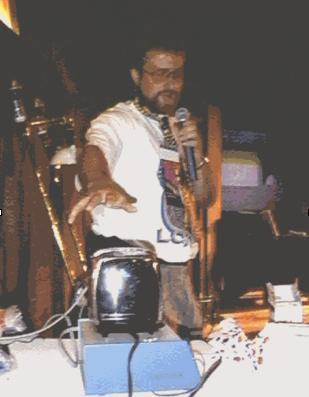
\includegraphics[scale=0.60]{immagini/toaster.jpg}
\caption{\textit{Simon Hackett presenta il toaster al pubblico}}
\end{figure}
\vspace{1.0cm}
Un altro primitivo esemplare di smart object viene sviluppato nel 1993 all'Università di Cambridge, il Trojan Room Coffee Pot. Si tratta di una caffettiera situata nella Trojan Room, una parte del Computer Laboratory dell'università, collegata ad una fotocamera in grado di catturare un'immagine della caffettiera per avere una stima della quantità di caffè rimanente. Sebbene oggi la cosa sembri banale all'epoca era piuttosto complesso catturare un frame, elaborarlo e renderlo disponibile su Internet tramite web service. Un server posto nel laboratorio difatti acquisiva ogni 3 minuti un'immagine ad alta risoluzione dalla fotocamera, la scalava e la rendeva disponibile tramite un meccanismo RPC (Remote Procedure Call) denominato MSRPC2, che a sua volta funzionava grazie ad uno strato network studiato appositamente per reti ATM proprio al Computer Laboratory, il MSNL (Multi-Service Network Layer). Infine un client, che fungeva anche da web-server per l'esterno, interrogava su richiesta il server RPC da cui otteneva l'ultimo frame catturato.
\\Nasceva così anche la prima webcam.
\\Daniel Gordon, il padre del progetto, affermò che il sistema fu inizialmente pensato per smascherare i "ladri di caffè" che da altre facoltà limitrofe venivano, durante la notte, a bere il caffè della facoltà di Informatica, che era risaputamente il più buono.
\\La webcam rimase attiva e perfettamente funzionante sino al 2001, quando venne smantellata.
\begin{figure}[!htbp]
\centering
\begin{minipage}[c]{.40\textwidth}
\centering
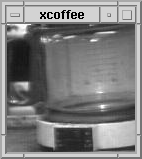
\includegraphics[width=.40\textwidth]{immagini/coffee-pot.png}
\caption{Un frame della caffettiera}
\end{minipage}%
\hspace{15mm}%
\begin{minipage}[c]{.40\textwidth}
\centering
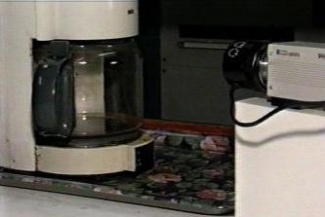
\includegraphics[width=.70\textwidth]{immagini/trcp.jpg}
\caption{Il sistema per catturare le immagini}
\end{minipage}
\end{figure}
\vspace{1.0cm}
\\Nel 1995 la Siemens sviluppa un modulo GSM chiamato "M1" disegnato specificatamente per comunicazioni M2M (Machine-to-Machine).
\\Nel 1998 nasce lo standard Bluetooth, oggi largamente utilizzato nello sviluppo di applicazioni e dispotivi IoT.
\\Nel 1999 Andy Stanford-Clark di IBM e Arlen Nipper di Arcom (ora Eurotech) presentano al pubblico il primo protocollo specifico per le comunicazioni M2M: MQ Telemetry Transport (MQTT), diventato un pilastro dell'Internet of Things e ancora oggi ampiamente diffuso.
\\Nel 2000 LG lancia sul mercato il primo frigorifero connesso alla rete, l'Internet Digital DIOS. Il frigorifero era in grado di rilevare, seppur con forti limitazioni, le quantità dei prodotti impostati e notificare l'esaurimento di questi. Sebbene questo prodotto ebbe un forte impatto sulla consapevolezza dell'evoluzione tecnologica che si stava affacciando, venendo addirittura citato in film di Hollywood, non ebbe particolare fortuna in quanto a vendite, probabilmente per via del suo prezzo proibitivo (al lancio costava oltre 20'000 \$) e del fatto che c'era scarsa fiducia in una tecnologia che era evidentemente prematura.
\\Nello stesso anno escono i primi dispositivi muniti di Bluetooth.
\\Negli anni a seguire, dal 2001 al 2005 circa, il termine Internet of Things diventa sempre più autorevole e viene citato sempre più spesso anche da importanti testate giornalistiche, sino addirittura a divenire protagonista, nel 2005, dell'annuale report redatto dall'ITU (International Telecommunication Union), l'agenzia delle Nazioni Unite che si occupa del monitoraggio delle tecnologie per la comunicazione.
\\Ritengo opportuno citare, sempre nel medesimo anno, la nascita del progetto tutto italiano Arduino, a cura di Massimo Banzi e di un team di studenti e ricercatori presso l'Interaction Design Institute di Ivrea. Il progetto Arduino, nel suo complesso, è stato negli anni a seguire un valido banco di prova per molti altri progetti di IoT, oltre ad essere un importantissimo strumento didattico.
\\\\Nel 2008 si capisce che la crescita e la diffusione degli smart objects ha bisogno di essere integrata con le tecnologie esistenti per formare reti interoperabili e nasce quindi la IPSO Alliance (Internet Protocol for Smart Objects), un consorzio di aziende che promuove l'utilizzo dello standard TCP/IP e in particolare del protocollo IP per la comunicazione con e tra smart objects.
\\\\Dal 2010 ad oggi l'IoT ha subito una incredibile accellerazione e diversi sono stati gli eventi importanti, tra cui è importante citare la nascita di Bluetooth Low Energy, con l'avvento dello standard Bluetooth 4.0, il lancio di IPv6, sempre più protagonista delle connessioni smart e non, la comparsa di altri protocolli applicativi per la comunicazione M2M, come CoAP e il lancio di prodotti che hanno segnato la storia del mondo smart come Nest e i Google Glass.


\section{Alcune applicazioni}
Questa sezione riguarda le possibili applicazione dell'Internet of Things nella vita di tutti i giorni. Le applicazioni trattate sono casi reali o realistici di utilizzo delle tecnologie IoT per migliorare la qualità della vita.


\subsubsection{Home Automation}
Sicuramente una delle applicazioni più diffuse e una delle prime ad essere esplorate. L'Home Automation nasce dal concetto di \textit{domotica}, termine in uso sino a qualche anno fa ma ora superato, espandendone gli orizzonti e le capacità. L'obiettivo è quello di rendere le abitazioni "intelligenti", per diverse ragioni:
\begin{itemize}
\item Risparmio energetico
\item Sicurezza
\item Comodità
\item Risparmio economico
\end{itemize}
Grazie all'IoT è infatti possibile installare nella casa una rete di sensori in grado, per esempio, di rilevare quando dimentichiamo una luce accesa e di spegnerla, di integrarsi con sistemi fotovoltaici e attivare elettrodomestici particolarmente esosi di energia solo quando la produzione dell'impianto fotovoltaico è elevata oppure avvisarci quando i consumi stanno sforando un determinato budget che abbiamo impostato.
\\Sensori di movimento accurati e comunicanti possono essere in grado di rilevare movimenti sospetti quando siamo in vacanza e attivare sistemi di registrazione video, oppure possono attivare allarmi silenziosi e telefonarci per avvisarci dell'intrusione e chiudere automaticamente le porte quando ce ne dimentichiamo.
\\O ancora, è possibile avere sistemi di automatismo che aprono il cancello di casa quando rilevano la prossimità del nostro veicolo o preparare il caffè la mattina quando suona la sveglia, o meglio ancora attivare la nostra sveglia in anticipo se rilevano traffico intenso sulla strada che solitamente percorriamo per andare a lavorare e molto altro ancora.
\\Il tutto facilmente configurabile e consultabile dal nostro PC o dal nostro smartphone/tablet.
\begin{figure}[H]
\centering
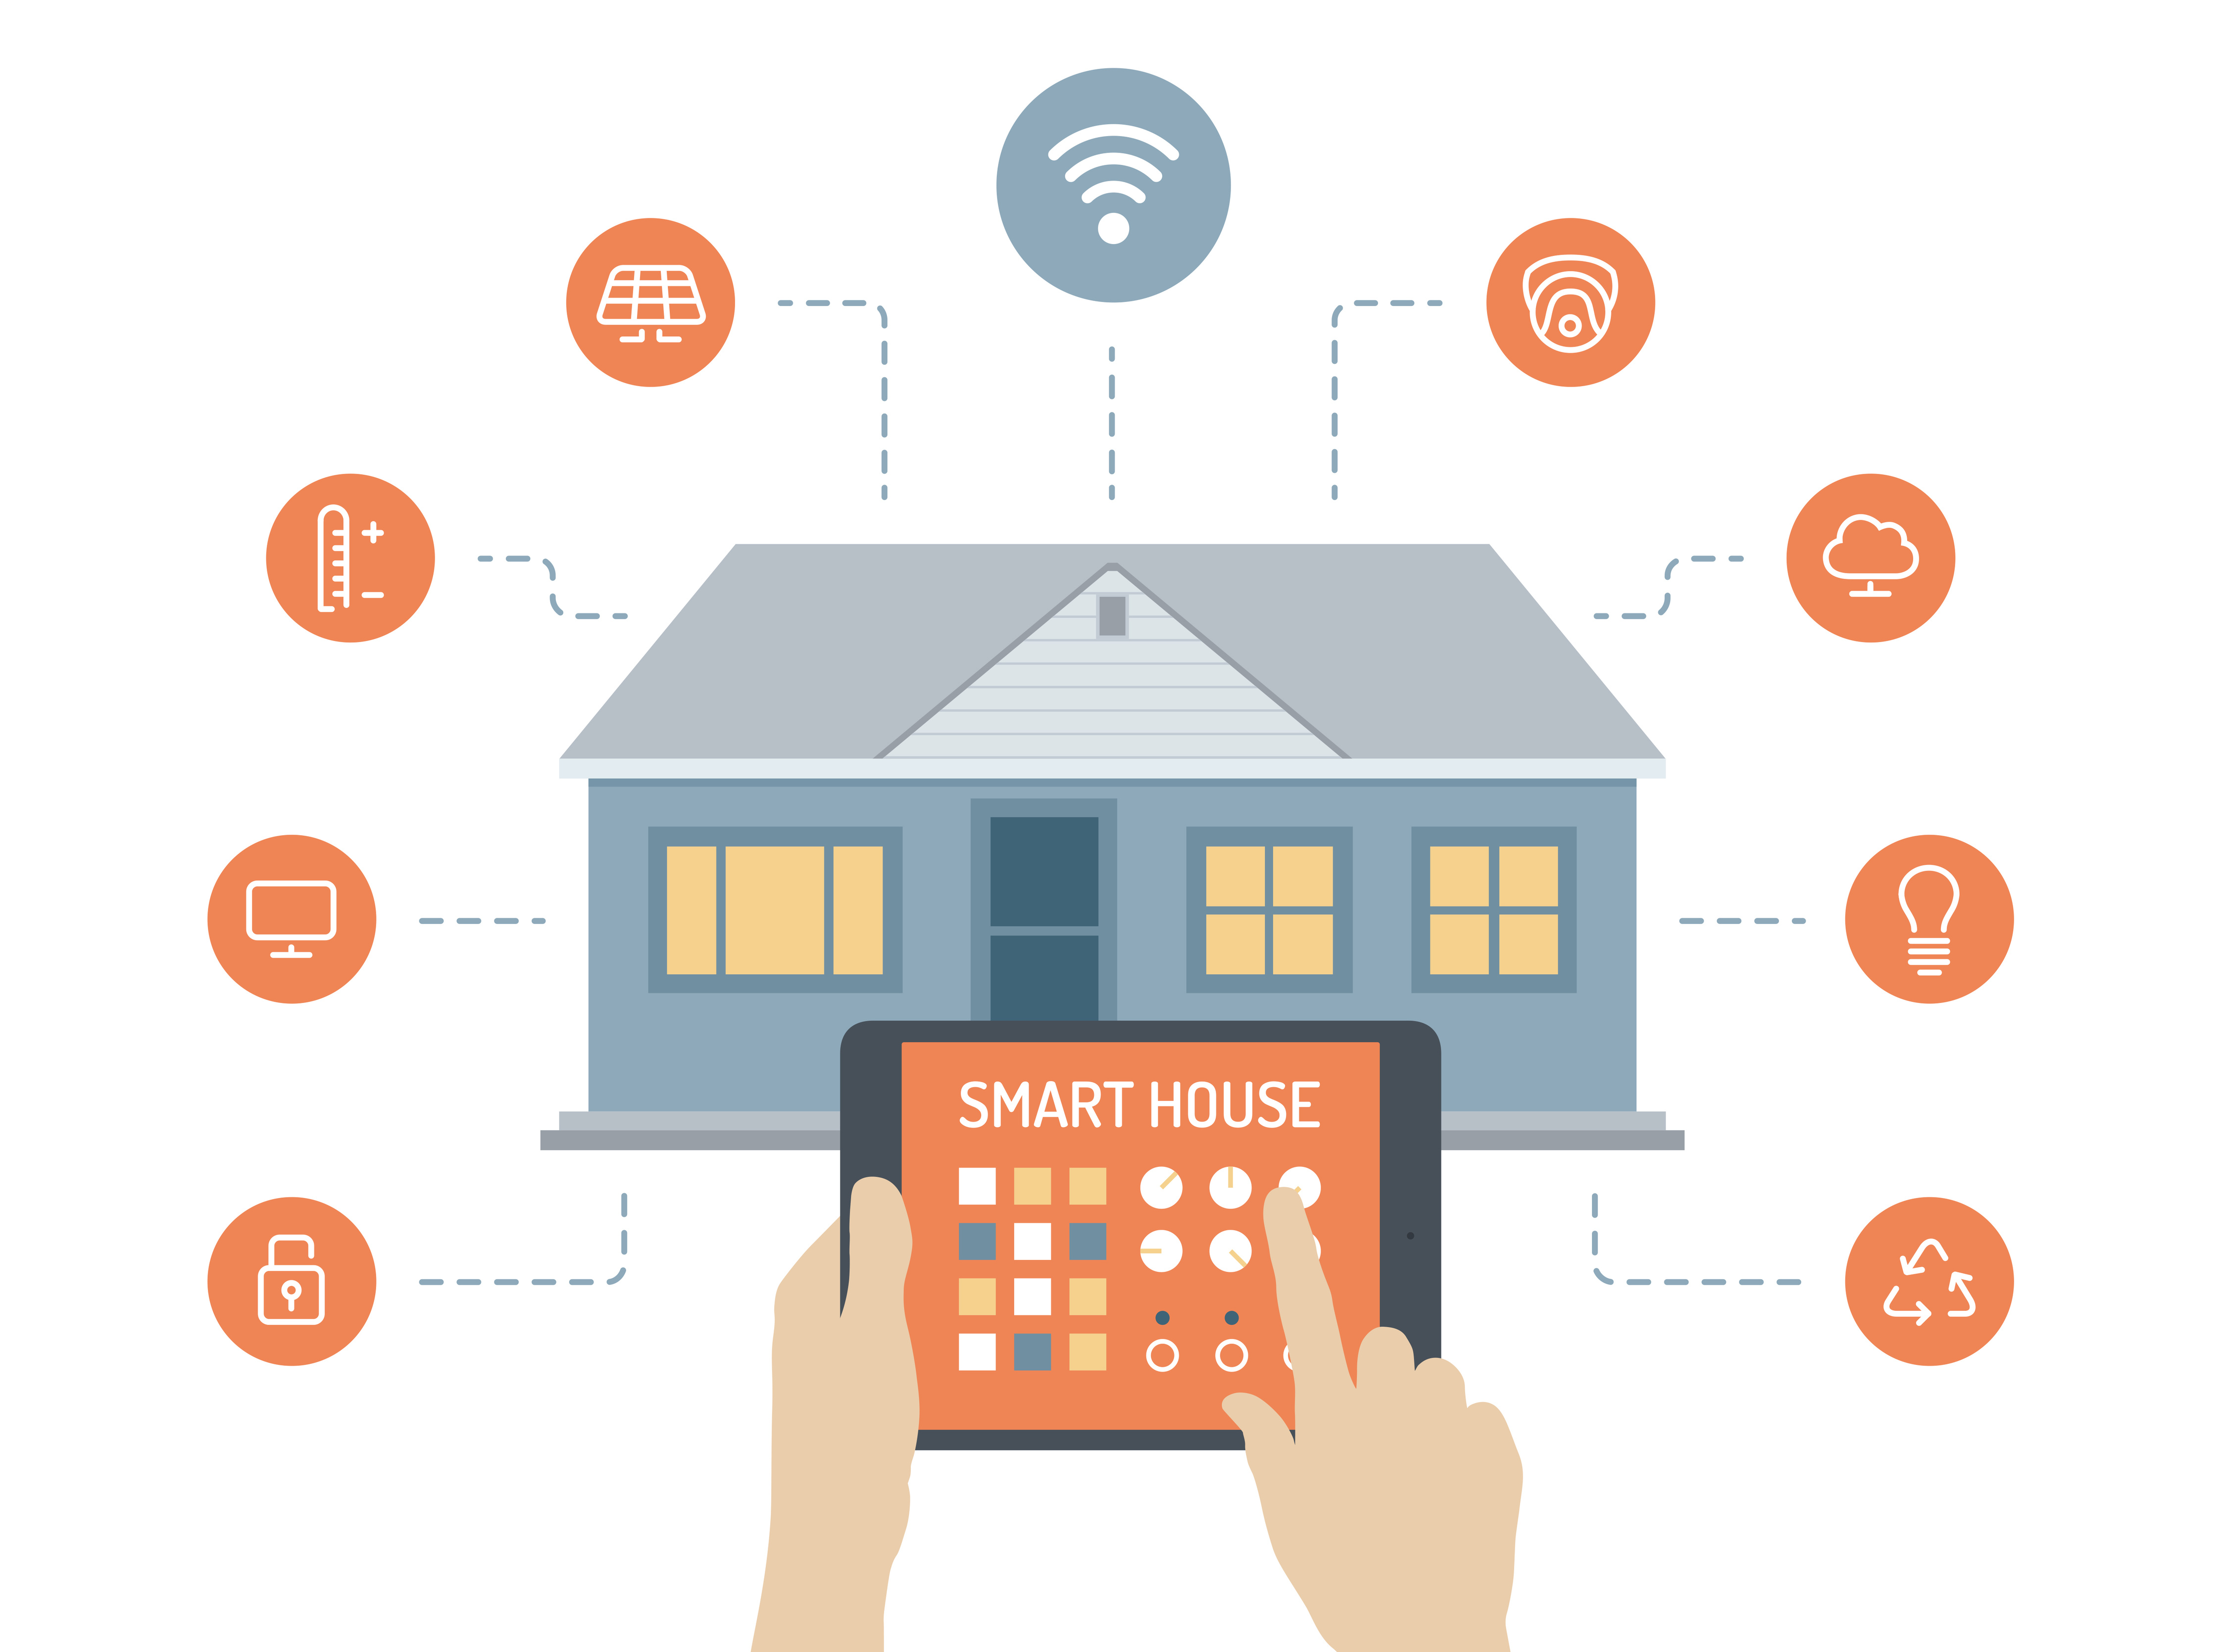
\includegraphics[scale=0.25]{immagini/Smart-Home.jpg}
\caption{\textit{Un esempio di smart home}}
\end{figure}

\subsubsection{Smart Metering}
Ambito più rivolto al Business che al Consumer, lo smart metering è il monitoraggio da parte di un dispositivo elettronico della corrente elettrica, del gas naturale o dell'acqua su intervalli prestabiliti. Il monitoraggio può essere effettuati su diversi fattori, come per esempio il consumo orario o la qualità dell'erogazione.
\\Questi sensori sono in grado, per esempio, di avvisare in caso di degradamento della qualità della corrente o dell'acqua, di offrire tariffe più vantaggiose in base alle nostre necessità di consumo e di fornire dati estremamente precisi alle aziende erogatrici. Lo smart metering è una realtà già da diverso tempo, anche qui in Italia: basti pensare ai contatori per l'energia elettrica installati nel 2002 da Enel Energia, in grado di monitorare i consumi e trasmetterli tramite linea elettrica (Powerline Communication) alla centrale più vicina.
\\Lo smart metering in realtà va anche oltre le stime strategiche utili alle aziende fornitrici dei servizi. Alcune città europee, come Parigi, stanno invitando i propri cittadini ad installare centraline di smart metering a casa propria che, inviando dati anonimi sull'utilizzo delle risorse, possono fornire una stima di come e quanto vengono utilizzate acqua corrente, energia elettrica e gas naturale nella città e migliorare di conseguenza i servizi e le forniture, oltre che promuovere programmi di risparmio energetico laddove i consumi siano elevati.
\\\\Una lodevole applicazione del concetto di smart meter è stata implementata dal consorzio FLEXMETER, che fa capo al Politecnico di Torino, supportato da grandi nomi quali IREN, TIM, STMicroelectronics, E.ON ed altri. Il progetto prevede la possibilità di installare dispositivi di smart metering all'interno di una piattaforma flessibile, in grado di integrarsi perfettamente con le tecnologie IoT presistenti. Il progetto è stato anche  finanziato dal programma di innovazione e ricerca dell'Unione Europea, Horizon 2020.
\begin{figure}[H]
\centering
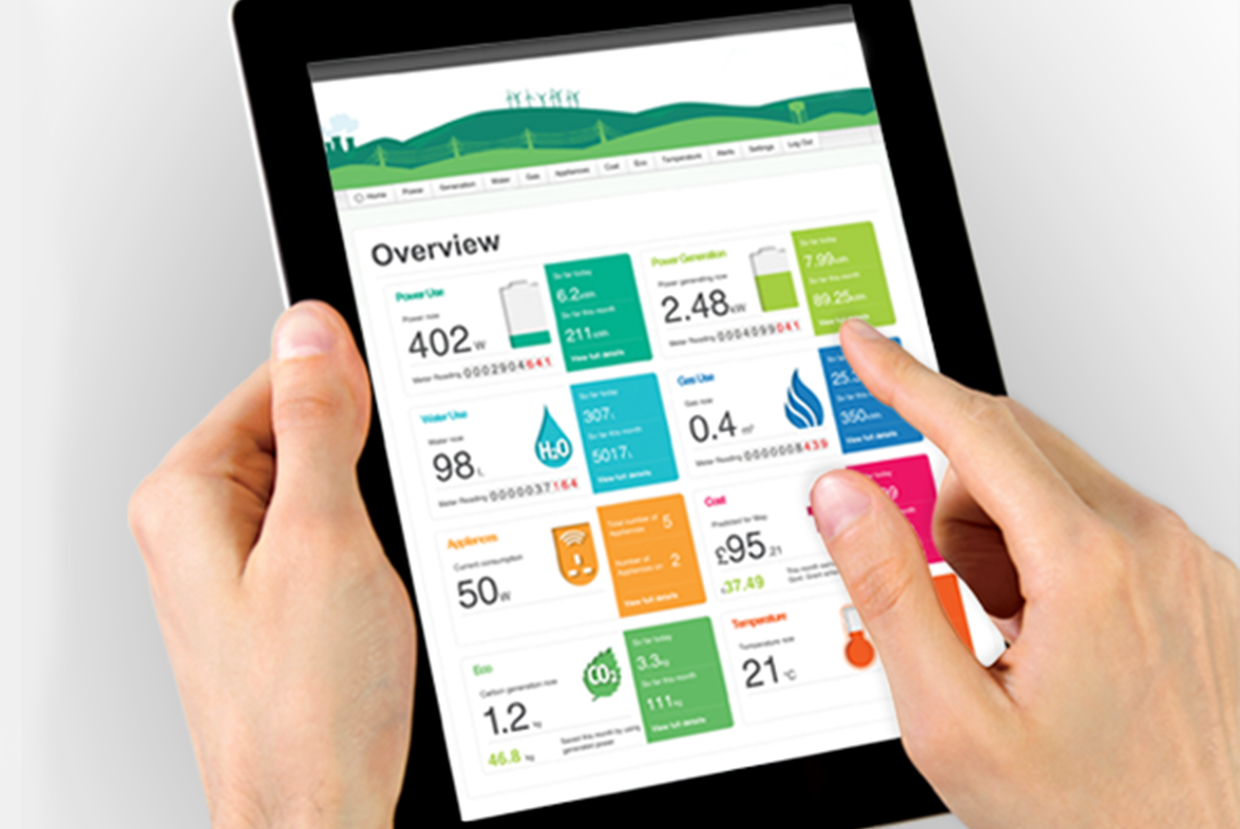
\includegraphics[scale=0.50]{immagini/Smart-Meter.png}
\caption{L'applicazione di monitoraggio FlexMeter}
\end{figure}

\subsubsection{Connected Vehicles}
Un altro interessante ambito applicativo dell'IoT lo possiamo ritrovare nel settore automotive, settore che indubbiamente gode di lauti finanziamenti in ricerca e sviluppo da parte dei costruttori. In particolare la ricerca in ambito Connected Vehicles si concentra sui cosiddetti "fattori umani", ovvero cercare di potenziare e/o limitare le capacità di guida umane. Sono nati quindi sistemi per rilevare ed allertare circa possibili ostacoli, ridurre intelligentemente le distrazioni visuali, assistere alla guida e al parcheggio e via dicendo.
Oltre ai sistemi di guida sono stati sviluppati anche sistemi di entertainment in grado di farci ascoltare la musica che preferiamo, in grado di avvisarci in caso di traffico e modificare l'itinerario e di operare perfettamente con altre tecnologie esistenti, quali smartphone e tablets.
\\Anche l'ambito sicurezza è stato oggetto di grande ricerca: sistemi di predizione e allerta di incidenti, sistemi di frenata automatica e schivamento di ostacoli ecc...
\\La sicurezza è e deve essere il tema più importante, e per questo molti governi ed enti di vigilanza hanno emanato regole ben precise sulla progettazione e sullo sviluppo di questi sistemi, imponendo certificazioni di qualità sia lato hardware che lato software alle aziende automobilistiche che vogliono operare entro i loro mercati.


\subsubsection{Smart Cities}
L'applicazione dell'Internet of Things alla realtà delle città nasce quasi contemporaneamente all'idea stessa di IoT. Innovare ed ottimizzare i servizi pubblici è diventato un obiettivo quasi obbligatorio, accellerato anche dalla recente crisi economica che ha messo in discussione alcune delle nostre abitudini. Le tecnologie dell'IoT vengono quindi impiegate per migliorare la mobilità, i consumi energetici, la gestione dei rifiuti e dell'ambiente in generale e in generale tutti quei servizi che incrementano la qualità di vita del cittadino all'interno della città. La città può quindi essere dotata di una rete di sensori wireless e wired che comunicano tra loro e verso sistemi di raccolta ed elaborazione dei dati. Si può, grazie a queste tecnologie, migliorare l'illuminazione pubblica, accendendo le luci solamente quando viene rilevato un soggetto che ne necessita, riducendo così gli sprechi. Oppure monitorare il traffico veicolare per poter produrre progetti urbanistici più efficienti, o ancora notificare agli automobilisti i parcheggi liberi a loro più vicini, permettendo non solo di ridurre il traffico ma anche le emissioni inquinanti. Sempre sull'inquinamento si può agire monitorando la qualità dell'aria e imponendo divieti di circolazione più mirati. I bidoni di raccolta dei rifiuti possono notificare quando sono pieni e necessitano di essere svuotati, ottimizzando la raccolta per evitare sprechi e migliorare il servizio e molto altro ancora.
\\Questi sensori possono essere inoltre integrati nella città per favorirne i servizi turistici o commerciali: alcuni esempi li possiamo trovare anche in Italia, come Mantova Phygital City, che ha creato alcuni punti di interesse ricchi di sensori e servizi in grado di dare al turista un'esperienza potenziata della città, o ancora Varese Smart City, progetto che tramite tecnologia NFC (Near Field Communication) è in grado di offrire al visitatore informazioni sugli eventi cittadini, sulle promozioni nei negozi, sulle attività commerciali che rispecchiano i gusti del visitatore stesso e sui luoghi di interesse.
\\\\Non è inoltre prematuro pensare che presto le reti domestiche e industriali possano essere completamente integrate all'interno di quelle cittadine, potenziando ulteriormente i servizi per il cittadino e per le imprese.
\begin{figure}[H]
\centering
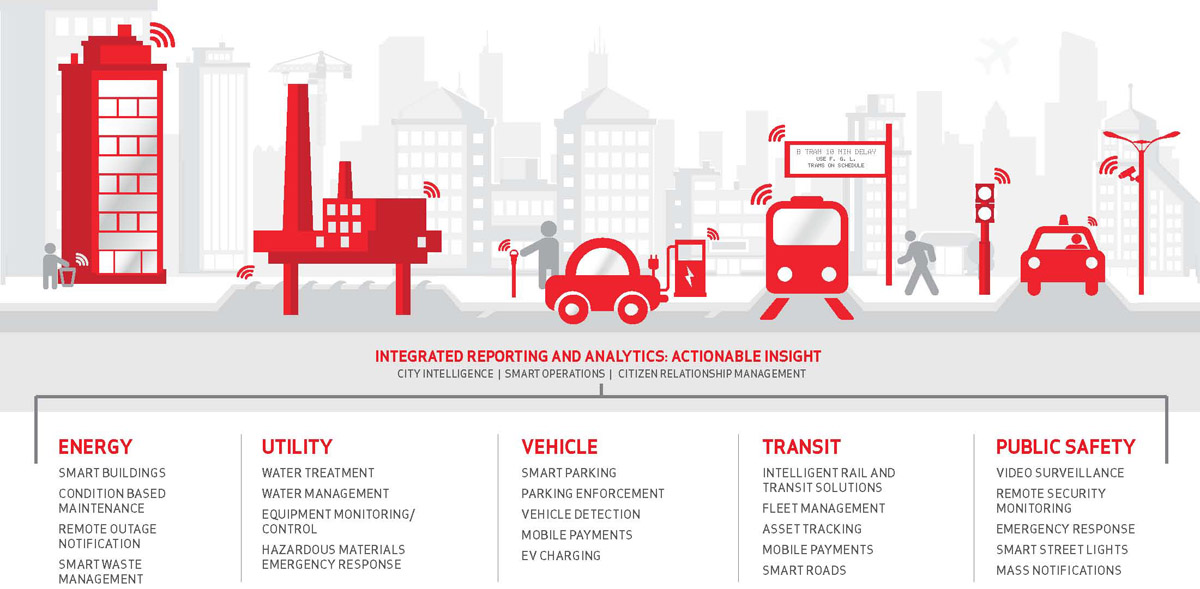
\includegraphics[scale=1.00]{immagini/Smart-City.jpg}
\caption{Un esempio di applicazione delle tecnologie smart all'interno della città}
\end{figure}

\subsubsection{Industrial \& Agriculture}
Settore certamente di grande rilievo e applicazione per l'IoT. L'Internet of Things ha riscontrato nel settore industriale e agricolo talmente tanto successo da aver dato il via, secondo alcuni esperti, alla quarta rivoluzione industriale, anche denominata Industria 4.0. L'idea è quella di creare, tramite smart objects, una rete in grado di potenziare e ottimizzare al massimo la produttività dell'azienda, riducendone i costi di produzione e di manodopera e aumentandone, quando possibile, la qualità.
\\Le tecnologie IoT vengono quindi utilizzate in ogni fase della produzione, a partire dall'ingegnerizzazione dei processi produttivi, dove, grazie ai rilevamenti effettuati nel tempo dalla rete sensoriale, si è in grado di creare modelli virtuali dell'azienda, rendendo possibile simulare modifiche ai processi produttivi e valutandone le conseguenze senza dover necessariamente cambiare la catena produttiva reale.
\\Si è inoltre in grado di valutare in tempo reale le condizioni di rendimento dell'azienda, di offrire servizi produttivi automatizzati anche all'esterno e di interoperare allo stesso modo con altre aziende che offrono a noi particolari servizi.
\\\\Più concretamente possiamo trovare sistemi in grado di avvisarci quando una linea produttiva ha un calo di rendimento, permettendo di identificare preventivamente guasti che metterebbero fuori uso per giorni la linea stessa, o addirittura sistemi in grado di auto-diagnosticare guasti e ripararsi da soli, oppure sistemi che sono in grado di controllare la qualità effettiva di un prodotto e scartarlo in automatico in caso di difetti.
\\O ancora, in ambito agricolo, possiamo trovare sensori che monitorano il terreno controllando l'irrigazione e la distribuzione di pesticidi solo quando è strettamente necessario, riducendo gli sprechi. Oppure sistemi di monitoraggio delle specie faunistiche presenti nelle piantagioni, per ottimizzare le lotte integrate e permettere ai prodotto biologici di essere competitivi.
\\\\Secondo Roland Berger, un'importante società di consulenza strategica, saranno necessari, per la sola Europa, investimenti intorno ai 90 miliardi di euro l'anno per 15 anni, per un totale di 1,350 bilioni di euro, per poter far partire correttamente l'Industria 4.0 e tornare ad essere competitivi sui mercati emergenti.


\subsubsection{Wearables \& Health Care}
Se l'IoT ha trovato grande successo nelle grandi reti di sensori non è certamente da meno il settore dei dispositivi indossabili. Già oggi stanno proliferando devices indossabili in grado di fornire informazioni dettagliate sullo stato di salute dell'indossatore, per esempio, o di tracciare un determinato itinerario seguito o ancora di fornire dati sulla qualità del sonno, monitorando i movimenti e le attività notturne del soggetto. Questi dispositivi trovano molteplici applicazioni e sono alla base dell'IoT più comune, più vicino al consumatore. Si potrebbe pensare a sistemi ospedalieri in grado di rilevare i parametri vitali di un paziente in tempo reale o di tracciarne la posizione anche all'interno dell'ospedale. O bracciali in grado di monitorare anziani affetti da Alzheimer, in grado di avvisare personale sanitario o parenti in caso di pericolo, notificando per esempio l'ultima posizione conosciuta del soggetto.
\\I progetti in tal senso stanno fiorendo negli ultimi anni, anche grazie al fatto che è possibile sviluppare dispositivi di questo tipo senza bisogno di ingenti fondi, facilitando le startup che ogni giorno apportano al settore costante innovazione.
\begin{figure}[H]
\centering
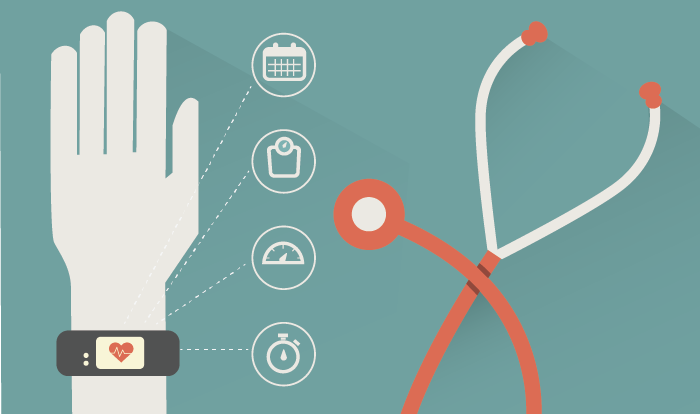
\includegraphics[scale=0.40]{immagini/wearable.png}
\caption{\textit{Un esempio di wearable per l'health care}}
\end{figure}

\chapter{I protocolli per l'IoT}
Parallelamente agli sviluppi tecnologici nel mondo dell'elettronica si è posto il problema di trovare protocolli di comunicazione adeguati che potessero permettere agli smart objects di comunicare tra loro e verso interfacce di più alto livello, rispettando le limitazioni imposte da una spesso ridotta capacità computazionale o di autonomia energetica.


\section{Il livello Data Link}
In questo paragrafo saranno trattati i protocolli del livello Data Link applicati all'IoT. Grandi protagonisti in questo ambito sono i protocolli radio, data la natura indipendente e mobile degli smart objects, che permettono ai dispositivi di comunicare senza avere necessità di collegamenti ingombranti e poco utili. Le frequenze trasmissive sono solitamente quelle ISM (Industrial, Scientific and Medical), porzioni dello spettro elettromagnetico non commerciali e che possono essere liberamente utilizzate, rispettando le potenze trasmissive imposte dai singoli Paesi. Troviamo quindi spesso protocolli che utilizzano le frequenze intorno ai 2,4 GHz come 802.15.4, WiFi (nei suoi standard b/g), Bluetooth, ANT+ ecc...
\\Queste frequenze garantiscono una discreta immunità da interferenze, la possibilità di utilizzare antenne ridotte e una buona larghezza di banda, anche se una scarsa penetrabilità degli ostacoli, il che limita solitamente il raggio utile a non più di 100 metri, a seconda della modulazione utilizzata.
\\\\Proprio per via dello scarso raggio d'azione ultimamente si stanno affacciando anche protocolli che operano nelle frequenze Sub-GHz, ovvero al di sotto del GHz, solitamente sfruttando le frequenze 868-915 MHz. L'utilizzo di frequenze più ridotte permette di trasmettere segnali ad una distanza maggiore, anche fino a 500-1000 Km, mantenendo pressochè uguali le potenze di trasmissione ma sacrificando il data rate. Alcuni network operativi sulle frequenze Sub-1GHz stanno nascendo per dare la possibilità agli smart objects di connettersi direttamente alla rete Internet senza bisogno di infrastrutture di supporto. Tra questi ricordiamo i più importanti, LoRa e SigFox, di cui parleremo successivamente.

\subsection{802.15.4 e ZigBee}
Tra i protocolli radio che maggiormente hanno trovato successo nel mondo IoT sicuramente 802.15.4, e le sue commercializzazioni, è uno di quelli che spicca maggiormente. Come tutte le reti appartenenti alle specifiche IEEE 802.15.x si tratta di un protocollo sviluppato per reti wireless a stretto raggio di copertura del segnale e con basse velocità di trasferimento, ovvero reti LR-WPAN (Low Rate Wireless Personal Area Network).
\\In questo ambito le applicazioni che vogliono utilizzare queste specifiche hanno richieste di:
\begin{itemize}
\item Bassi costi
\item Bassa complessità di implementazione
\item Scarsi consumi energetici, ovvero ampia durata di eventuali batterie
\item Data rate modesti
\end{itemize}
Le topologie di rete previste in questo standard sono due, a stella e peer-to-peer, e con due differenti tipologie di dispositivi partecipanti: Full Function Device (FFD) e Reduced Function Device (RFD). Gli RFD sono tipicamente dispositivi a scarsa o scarsissima potenza computazionale che sono in grado di svolgere funzioni basiche e pertanto possono comunicare solamente con dispositivi FFD, i quali si occuperanno, se necessario, di smistare i messaggi verso altri RFD o verso dispositivi di più alto livello.
\\Nella topologia a stella troviamo un nodo FDD centrale che funge da \textit{PAN Coordinator}, ovvero smista i pacchetti provenienti dai nodi RFD e comunica con altri nodi FDD che però non hanno ruolo di coordinatori. In questa topologia è il \textit{Coordinator} che per primo comunica agli altri nodi l'identificativo della rete, rendendo la rete completamente indipendente da eventuali altre reti presenti.
\\Nella topologia peer-to-peer, invece, il primo device FDD che trasmette diventa \textit{Coordinator} ma in qualunque momento un nodo FDD può assumere quel ruolo per coordinare nodi RFD che sono collegati a lui e instradare il messaggio sulla rete. 802.15.4 non definisce alcun protocollo di routing per questa topologia di rete, demandando il compito agli strati superiori.
\\\\La modalità di accesso al canale è CSMA/CA (in versione "semplificata"), mentre per la trasmissione si utilizzano tecnologie \textit{Spread Spectrum} per ridurre le interferenze.
\\Le frequenze solitamente utilizzate sono le classiche 2.4 GHz, ma in realtà talvolta 802.15.4 viene utilizzato su frequenze Sub-1Ghz, in particolare 868 e 915 MHz e, con le ultime revisioni dello standard, è stata introdotta anche la possibilità di utilizzare frequenze a 5 GHz, molto più libere da interferenze.
\\I data-rates supportati sono 250, 40 e 20 kb/s e il raggio utile di trasmissione non supera i 30-40 metri.
\\\\Il pacchetto 802.15.4, a livello PHY (\textit{Physical}) è formato da:
\begin{itemize}
\item \textbf{Preamble}: 4 byte di lunghezza, utilizzato per la sincronizzazione
\item \textbf{Start of Packet Delimiter}: 8 bit di lunghezza, utilizzato anche questo per sincronizzare la comunicazione
\item \textbf{PHY Header}: 1 byte, contenente il campo \textit{Frame Length} di 7 bit più 1 bit riservato per usi futuri.
\item \textbf{PHY Service Data Unit (PSDU)}: da 0 a 127 byte di lunghezza, contenente a sua volta il pacchetto MAC.
\end{itemize}
Il pacchetto dello strato MAC è articolato ma è interessante notare come l'indirizzamento preveda un indirizzo univoco da 64 bit per ogni dispositivo sulla stessa rete PAN e quindi, potenzialmente, circa 18 trilioni di dispositivi per ogni network.
\\Tuttavia al momento dell'associazione alla rete il \textit{Coordinator} assegna al device uno \textit{short-address} da 16 bit, limitando quindi l'indirizzamento a 65'535 dispositivi, numero comunque sufficiente a coprire ampiamente le esigenze odierne.
\begin{figure}[!h]
\centering
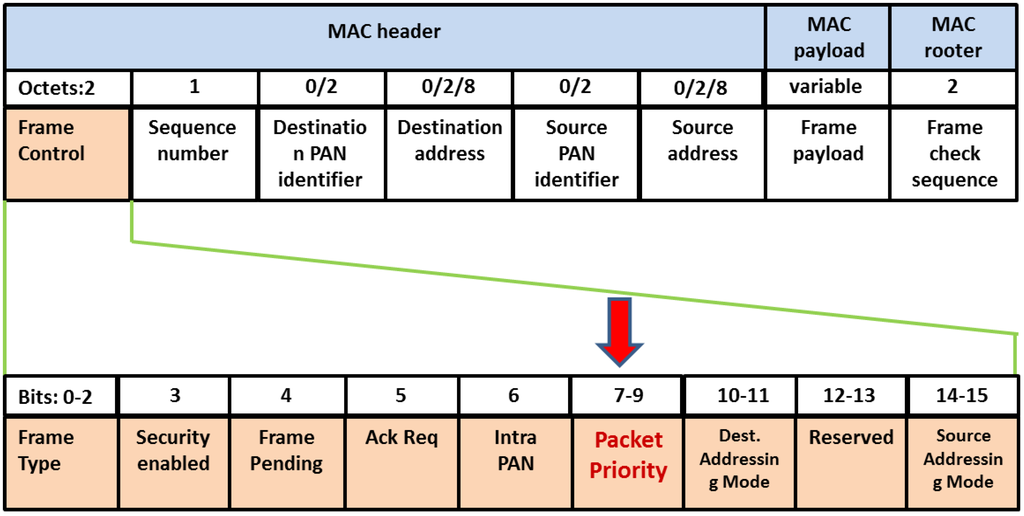
\includegraphics[scale=3.00]{immagini/802154-frame.png}
\caption{\textit{Il frame 802.15.4, sia a livello fisico che a livello MAC}}
\end{figure}
802.15.4 è in grando inoltre di sfruttare tecniche di accesso al canale e trasmissione/ricezione sincronizzate per ottimizzare al massimo il risparmio energetico, importante richiesta di questa tipologia di dispositivi, e prevede dei meccanismi di sicurezza integrati nello strato MAC, per fornire integrità, autenticazione e confidenzialità ai messaggi, pur mantenedo un basso profilo energetico.
\vspace{1.0cm}
\\Sopra lo standard 802.15.4 sono state costruite diverse "commercializzazioni" e standard operanti sui livelli più alti dello stack ISO/OSI. Uno dei più famosi e largamente utilizzati è certamente \textbf{ZigBee}, nato nel 2004 e giunto ora alla sua terza specifica. ZigBee prevede tre possibili tipologie di dispositivi partecipanti:
\begin{itemize}
\item \textit{ZigBee Coordinator}: coincide in tutto e per tutto con l'omonimo ruolo della specifica 802.15.4, ovvero si occupa di "creare" la rete, memorizzare eventuali chiavi di sicurezza e può operare da ponte tra più reti. Ci può essere un solo \textit{Coordinator} per ogni rete.
\item \textit{ZigBee Router}: questa tipologia di dispositivi permette di scambiare pacchetti tra i dispositivi o tra porzioni della stessa rete, effettuando anche multi-hopping, ovvero ritrasmissione e routing.
\item \textit{ZigBee End Device}: sono i dispositivi a funzionalità minime, possono dialogare solo con i \textit{Coordinator} o con i \textit{Router} e non partecipano al multi-hop di un messaggio.
\end{itemize}
Il protocollo di routing solitamente utilizzato è l'AODV (\textit{Ad-hoc On-demand Distance Vector}, un algoritmo derivato dal classico \textit{Distance Vector} ma pensato per reti mobili e dove le trasmissioni devono essere limitate al minimo. AODV, a differenza di Distance Vector classico, interviene a calcolare il percorso di routing solo quando richiesto, ovvero quando si cerca di accedere ad un nodo di cui ancora non si conosce il percorso; questo limita notevolmente il traffico per percorsi già stabiliti anche se aumenta considerevolmente il tempo di risposta nel caso il routing sia ancora sconosciuto. AODV supporta anche instradamenti di tipo unicast e multicast.

\subsection{Altri}

\section{I livelli di rete e trasporto}

\subsection{IPv6 e lo strato 6LoWPAN}
\subsection{UDP}


\section{Il livello applicativo}

\subsection{CoAP}
\subsection{Altri}

\chapter{Architettura e sviluppo del sistema}
Come esposto nei capitoli precedenti, le reti IoT nascono con l'intenzione di mettere in comunicazione potenzialmente milioni di sensori e dispositivi. Questi dispositivi possono avere interfacce differenti, avere hardware differente e possono assolvere a compiti completamente differenti l'uno dall'altro. L'obiettivo è quello di sviluppare un sistema centralizzato in grado di monitorare questi smart objects, su richiesta dell'utente, e pubblicare cambiamenti di stato o valori periodici su canali familiari all'utente, che può consultare con semplicità.
\\Il sistema deve necessariamente essere strutturato considerando le seguenti parole chiave:
\begin{itemize}
\item \emph{Scalabilità}: data la potenziale mole di nodi da osservare è mandatorio che il sistemi scali correttamente.
\item \emph{Portabilità}: il sistema deve essere slegato da vincoli hardware e soprattutto software relativi ai sistemi operativi, data la molteplicità di realtà presenti oggi sul mercato, potendo potenzialmente essere portato in sistemi cloud più estesi.
\item \emph{Interoperabilità}: il sistema deve necessariamente essere interoperabile, ovvero deve poter operare con il maggior numero possibile di nodi e dispositivi, cercando di astrarre il più possibile dal tipo di dati trattati e dalle sue caratteristiche intrinseche. Il sistema deve inoltre essere in grado, potenzialmente, di poter restituire i dati su differenti canali ed essere sempre pronto all'espansione e alle modifiche in tal senso.
\end{itemize}
Il sistema sarà quindi composto da tre unità fondamentali:
\begin{itemize}
\item La cloud Java
\item Il DBMS
\item L'interfaccia Web
\end{itemize}
Tutte le componenti sono state pensate e sviluppate per poter essere indipendenti e intercambiabili, nei limiti del possibile, per ottenere un sistema flessibile e facilmente manutenibile.
\vspace{1.0cm}
\begin{figure}[h]
\centering
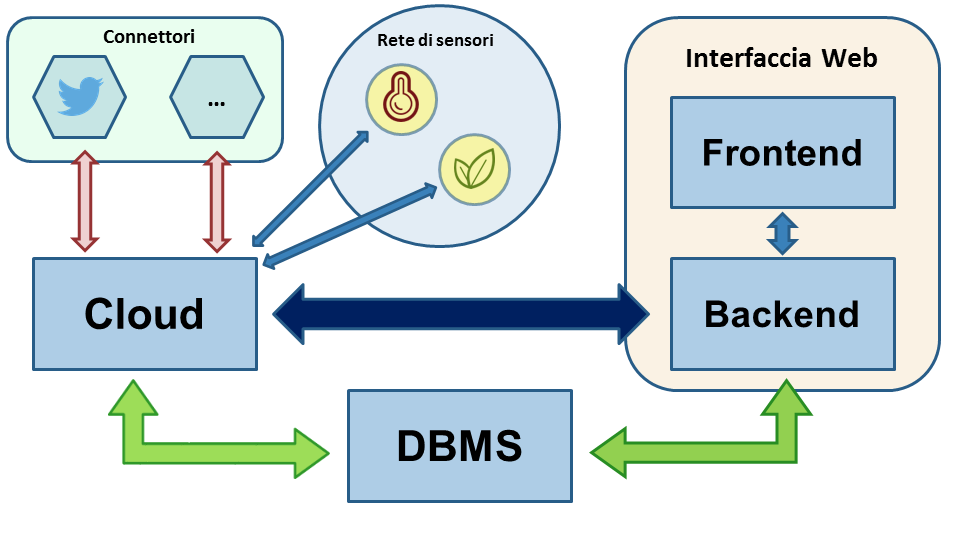
\includegraphics[width=\textwidth]{immagini/cloud.png}
\caption{\textit{L'architettura del sistema di monitoraggio}}
\end{figure}

\section{La cloud Java}
La cloud Java è certamente la componente più importante dell'intero sistema: essa si occupa infatti di effettuare il monitoraggio delle risorse tramite protocollo CoAP su richiesta dell'interfaccia Web, e di pubblicare, periodicamente o al succedersi di un evento, i dati ottenuti su canali definiti dall'utente, chiamati \textit{connettori}.
\\Le richieste dall'interfaccia Web verso la cloud sono fatte mediante chiamate remote, utilizzando XML-RPC.
\\È stato scelto il linguaggio Java principalmente per la sua caratteristica intrinseca di portabilità: è infatti sufficiente avere la JVM (Java Virtual Machine) per far girare la cloud, non essendoci chiamate particolari al sistema operativo e non effettuando alcuna operazione dedicata su hardware specifico. Il linguaggio Java inoltre, grazie al livello di astrazione eccezionale che fornisce, ha permesso uno sviluppo veloce e abbastanza ordinato, anche grazie all'ampia disponibilità di librerie, sia integrate che facilmente reperibili da terze parti. 
\\La cloud è sostanzialmente composta da un server XML-RPC, la classe {\tt Server}, che è sempre in esecuzione e disponibile, che riceve le chiamate remote dall'interfaccia; a questo punto le chiamate vengono passate all'handler XML-RPC, la classe {\tt CoapHandler}, che a sua volta le smista al {\tt CoapAgent}, un thread particolare di cui esiste una sola istanza, che è un po' l'esecutore materiale della richiesta: si occupa infatti di creare l'azione richiesta nel database, configurare il connettore e lanciare il thread specifico che si occuperà di monitorare la risorsa indicata dall'utente. L'{\tt Agent} ha anche il compito di interrompere l'esecuzione di questi thread di monitoraggio se richiesto e, anche se in piccola parte, si occupa di controllare che ogni thread non sia "pendente", ovvero che non sia rimasto in esecuzione nonostante la sua azione non sia più presente nel database.
\begin{figure}[hp]
\centering
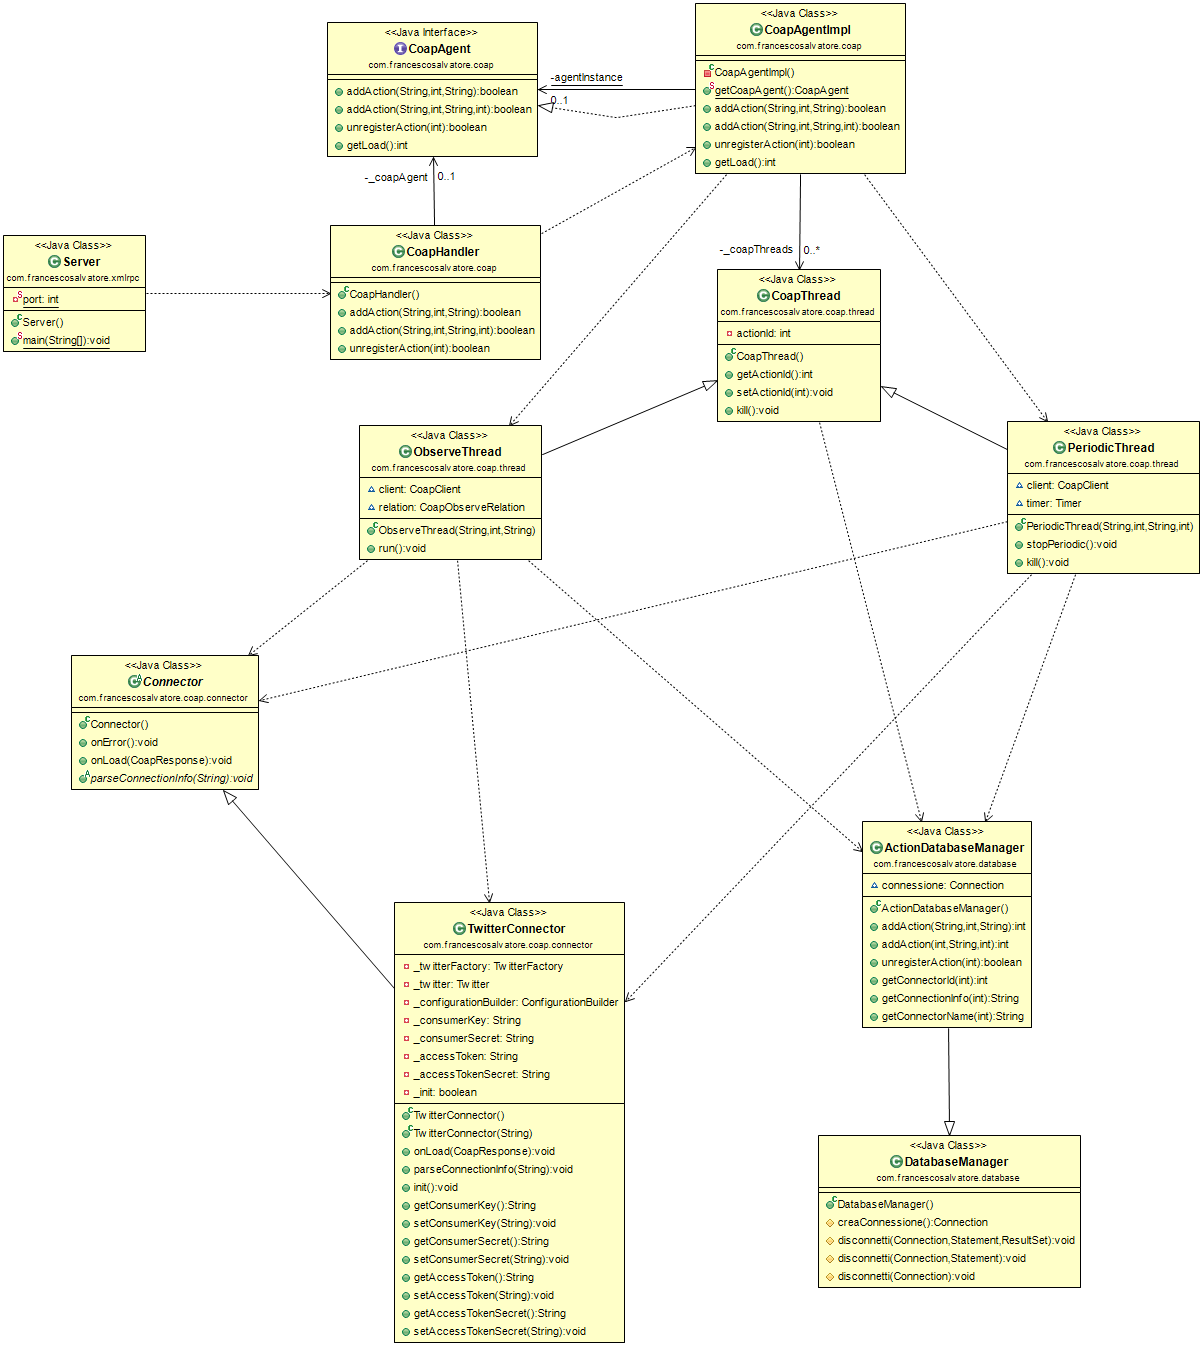
\includegraphics[width=\textwidth]{immagini/uml.png}
\caption{\textit{Il diagramma UML delle classi della cloud Java}}
\end{figure}
\vspace{1.00cm}
Possiamo trovare due tipi, per il momento, di thread di monitoraggio:
\begin{itemize}
\item {\tt ObserveThread}: si mettono in ascolto su di una risorsa e, in caso di cambiamento di evento sulla risorsa, lo notificano al connettore scelto.
\item {\tt PeriodicThread}: controllano periodicamente il valore della risorsa indicata, secondo il tempo richiesto dall'utente, e notificano il valore al connettore scelto.
\end{itemize}
I connettori quindi ricevono il valore e lo elaborano, a seconda del comportamento del connettore stesso.
\\\\Il DBMS scelto è MySQL, per alcune semplici ragioni: è gratuito, nella sua versione base, è semplice da installare ed è multipiattaforma, oltre che essere conforme agli standard ANSI SQL e ODBC SQL. Per la connessione e la gestione è stato però scelto di utilizzare il driver \textit{JDBC} (Java DataBase Connectivity), che permette di creare un livello di astrazione tra le chiamate al database e il database stesso, garantendo la possibilità di poter cambiare DBMS con semplicità e in maniera "indolore", senza quindi dover radicalmente modificare la struttura o il codice stesso del programma. Questo accorgimento ci permette di poter spaziare tra i DBMS che supportano ODBC e per i quali esiste il driver specifico, tra i quali troviamo i maggiormente utilizzati PostgreSQL, Oracle, Microsoft SQL Server, Sybase, DB2, SQLite e molti altri.
\\Vi è inoltre una classe che si occupa di implementare l'astrazione dal database, che è la classe {\tt DatabaseManager}.

%Server.java
\lstset{title=La classe Server}
\begin{lstlisting}[float]
public class Server {
	
	private static int port = 8008;
	
	public static void main(String args[])
	{
		try
		{
			WebServer server = new WebServer(port);
			XmlRpcServer xmlrpcserver = server.getXmlRpcServer();
			PropertyHandlerMapping phm = new PropertyHandlerMapping();
			phm.addHandler("coap", com.francescosalvatore.coap.CoapHandler.class);
			xmlrpcserver.setHandlerMapping(phm);
			server.start();
			System.out.println("CoAP Cloud Server running on port "+port+"...");
		}
		catch(Exception e)
		{
			System.out.println(e.getMessage());
		}
	}
}
\end{lstlisting}

%CoapAgent.java
\lstset{title=L'interfaccia CoapAgent}
\begin{lstlisting}[float]
public interface CoapAgent {
	
	/**
	 * Register an OBSERVABLE action on ResourceURI specified.
	 * @param actionName is the name of the action.
	 * @param connectionId is the identifier of connection in database.
	 * @param resourceURI is the URI that point to the observable resource.
	 * @return TRUE if action has been correctly created, FALSE otherwise.
	 */
	public boolean addAction(String actionName, int connectionId, String resourceURI);
	
	/**
	 * Register a PERIODIC action on ResourceURI specified.
	 * @param actionName is the name of the action.
	 * @param connectionId is the identifier of connection in database.
	 * @param resourceURI is the URI that point to the observable resource.
	 * @param period is the periodic time (in seconds). At each period the Agent send a GET request to the resource
	 * and perform the action request by connector.
	 * @return TRUE if action has been correctly created, FALSE otherwise.
	 */
	public boolean addAction(String actionName, int connectionId, String resourceURI, int period);
	
	/**
	 * @param actionId is the action identifier in database.
	 * @return TRUE if the action is unregistered, FALSE if an error has occurred.
	 */
	public boolean unregisterAction(int actionId);
	
	/**
	 * @return the number of running threads on this Agent. 
	 */
	public int getLoad();
}
\end{lstlisting}

%CoapAgent.java
\lstset{title=L'ObserveThread}
\begin{lstlisting}[float]
public class ObserveThread extends CoapThread {
	
	CoapClient client;
	CoapObserveRelation relation;
	
	public ObserveThread(String actionName, int connectionId, String resourceURI) throws SQLException, InvalidConnectorException
	{
		ActionDatabaseManager dbMan = new ActionDatabaseManager();
		int actionId = dbMan.addAction(actionName, connectionId, resourceURI);
		if(actionId == 0) throw new SQLException("Error during INSERT action in database.");
		this.setActionId(actionId);
		
		//Build correct handler from connector
		Connector connector;
		String connectionInfo = dbMan.getConnectionInfo(connectionId);
		switch(dbMan.getConnectorName(dbMan.getConnectorId(connectionId)))
		{
			case "Twitter":
				connector = new TwitterConnector(connectionInfo);
				break;
				
			default: 
				connector = null;
				throw new InvalidConnectorException("Connector name provided is not valid.");
		}
		
		this.client = new CoapClient(resourceURI);
		this.relation = client.observe(connector);
	}
	
	public void run()
	{
		try {
			for(;;) Thread.sleep(Long.MAX_VALUE);
		} catch (InterruptedException e) {
			e.printStackTrace();
		}
	}
}
\end{lstlisting}

Per la comunicazione verso le risorse, ovvero gli smart objects, è stato scelto il protocollo CoAP. CoAP è semplice, garantisce un basso overhead ed è in grado di funzionare adeguatamente sia su reti IPv4 che IPv6, garantendo una buona interoperabilità del nostro sistema e delle reti monitorate con infrastrutture e architettura già presenti. CoAP inoltre presenta la possibilità di "osservare" una risorsa, tenendo costantemente monitorato il suo valore ed essendo avvisati dalla risorsa stessa in caso di cambiamento, evitando alla cloud di dover effettuare un polling costante sulla risorsa stessa, che sarebbe eccessivamente gravoso sia in termini di risorse di calcolo sia in termini di traffico di rete generato (ricordiamo che spesso questi smart objects sono all'interno di reti a ristretta larghezza di banda ed effettuare polling costanti anche su pochi dispositivi significherebbe saturare queste reti).
\\La libreria che ci permette di effettuare queste operazioni su CoAP è Californium, un framework completo che permette di lavorare sia in modalità client che server, sviluppato da Matthias Kovatsch. Californium è passata con successo all'ETSI (European Telecommunications Standards Institute) IoT PlugTest, un test di interoperabilità tra sistemi di smart objects. Californium è potente ma allo stesso tempo leggero e facilmente gestibile. Inoltre permette di simulare smart objects su differenti reti, funzionalità che ho ampiamente utilizzato per emulare una rete di sensori.

\subsection{XML-RPC}
Considerando gli obiettivi del sistema di portabilità e interoperabilità era necessario pensare ad una modalità standard per poter mettere in comunicazione l'interfaccia Web e la cloud. È stata fatta quindi la scelta di utilizzare un sistema stile web-service, che garantisce di poter sostituire l'interfaccia Web o la cloud utilizzata con un qualunque sistema in grado di effettuare e ricevere chiamate remote. In particolare la scelta è caduta su XML-RPC, protocollo che utilizza il linguaggio XML per incapsulare le chiamate e HTTP come modalità di trasporto, per ragioni di semplicità: XML-RPC è infatti più semplice e leggero di altri sistemi RPC come SOAP, non necessita di definire encoding particolari e non necessita di creare le descrizioni del servizio WSDL (Web Service Description Language), superflue agli scopi di questo sistema.
\\Il funzionamento di XML-RCP è abbastanza elementare: le chiamate di funzione, con relativi argomenti, vengono serializzate in linguaggio XML, che viene poi passato al server tramite protocollo HTTP, che li deserializza. Questo meccanismo rende veramente agevole il processo di chiamata remote ed è estremamente compatibile con le tecnologie esistenti, in quanto sia XML che HTTP sono ampiamente supportati.
\\Esistono in fatti decine di implementazioni di questo protocollo ed è stato scelto di utilizzare la libreria \textit{Apache XML-RPC2} per quanto riguarda la cloud Java, mentre per l'interfaccia Web è stato scelto di utilizzare il modulo integrato in PHP (dalla versione 5.0 in su).

\subsection{I connettori}
Uno dei problemi dell'utilizzare reti di sensori estese è sicuramente quello di ottenere i dati in maniera semplice, chiara, leggibile anche da un utente consumatore senza particolare esperienza nel campo tecnologico, e certamente una delle funzionalità più interessanti è quella di essere avvisati dalla rete di sensori quando sussiste un determinato evento (un cambiamento di un valore di temperatura, oppure un movimento rilevato da un sensore di movimento ecc...). È quindi utile poter utilizzare canali comodi e familiari all'utente, come per esempio i social media, per pubblicare i dati e da qui l'idea di sviluppare il sistema modulare, pronto per impiantare sopra di esso dei \textit{connettori}, ossia delle interfacce di astrazione che si occupano di ricevere il dato grezzo ed elaborarlo, secondo la propria specifica: il connettore di Twitter, per esempio, potrebbe pubblicare un tweet, o quello di Facebook un messaggio sulla propria bacheca; o ancora un connettore per Telegram, la nota app di messaggistica, potrebbe inviarci un messaggio sul nostro smartphone oppure il connettore mail potrebbe inviare una email al nostro indirizzo personale e via dicendo.
\\La cloud Java offre quindi una interfaccia {\tt Connector} che definisce alcuni metodi e proprietà che ogni connettore deve avere, ma lascia ampia libertà implementativa, permettendo una customizzazione abbastanza elevata del comportamento del singolo connettore.
\\Nel sistema cloud in questione è stato implementato un solo connettore, quello di Twitter, che è in grado di pubblicare sulla propria timeline un tweet contenente il dato estratto dalla risorsa monitorata.

%TwitterConnector.java
\lstset{title=Parte della classe TwitterConnector}
\begin{lstlisting}[float]
public class TwitterConnector extends Connector {
	
	private TwitterFactory _twitterFactory;
	private Twitter _twitter;
	private ConfigurationBuilder _configurationBuilder;
	
	private String _consumerKey;
	private String _consumerSecret;
	private String _accessToken;
	private String _accessTokenSecret;
	
	private boolean _init = false;
	
	public TwitterConnector() {}
	
	public TwitterConnector(String connectionInfo)
	{
		parseConnectionInfo(connectionInfo);
		_twitterFactory = new TwitterFactory(_configurationBuilder.build());
		_twitter = _twitterFactory.getInstance();
		_init = true;
	}
	
	@Override
	public void onLoad(CoapResponse response)
	{
		if(!_init) return;
		try 
		{
			_twitter.updateStatus(response.getResponseText());
		} 
		catch (TwitterException e) {
			e.printStackTrace();
		}
	}

	...
	
	public void init()
	{
		_twitterFactory = new TwitterFactory(_configurationBuilder.build());
		_twitter = _twitterFactory.getInstance();
		_init = true;
	}
	
	...
}
\end{lstlisting}

\subsection{Le REST APIs e la libreria Twitter4J}
Twitter mette a disposizione degli sviluppatori una interessante API (Application Programming Interface) REST, ovvero una interfaccia HTTP che utilizza il modello URL per ricevere le richieste dall'applicazione e restituisce i risultati in formato JSON. Le Twitter APIs utilizzano un sistema di autenticazione denominato OAuth, ed in particolare la versione 2.0, un protocollo che permette di ottenere un discreto livello di sicurezza per ottenere dati particolari. Il protocollo OAuth è standardizzato ed è stato recepito da IETF nel RFC 6749.
\\Le REST APIs permettono, seppur con qualche limitazione, di effettuare operazioni sui dati Twitter ma necessitano di chiavi di autenticazione che solo l'utente stesso può fornire. In questo modo si garantisce che nessuna applicazione di terze parti possa, senza l'autorizzazione del proprietario dell'account, effettuare pubblicazioni a suo nome.
\\Per l'interfacciamento con le REST APIs è stato scelto di utilizzare la libreria \textit{Twitter4J}, sviluppata da Yusuke Yamamoto e distribuita sotto Apache License 2.0. La libreria permette di effettuare, direttamente da Java, chiamate alla API, supporta nativamente OAuth ed è semplice da integrare, non richiedendo alcuna dipendenza aggiuntiva.

\section{L'interfaccia Web}
Come è importante per l'utente poter accedere ai dati della rete di smart objects tramite canali a lui familiari, è altrettanto importante fornirgli una modalità di configurazione semplice ed intuitiva, che sia fruibile tramite il maggior numero possibile di dispositivi nei modi più chiari possibile.
\\È naturale quindi che sia stato scelto l'ambiente Web per lo sviluppo dell'interfaccia, in quanto altamente raggiungibile sia da dispositivi classici, come PC, sia da dispositivi mobili, come smartphone e tablet, sia da altre tipologie di dispositivi che sempre più sono equipaggiati con interfacce di rete e applicazioni browser, come smart TV, Set-top-box, console videoludiche ecc...
\\L'idea è quella, anche qui, di sviluppare un sistema di backend che sia altamente compatibile con il maggior numero possibile di architetture e sistemi, che sia scalabile e facilmente manutenibile.
\\Sebbene inizialmente sia stato preso in considerazione di sviluppare l'interfaccia Web al di sopra della cloud, sfruttando tecnologie offerte dall'ambiente Java come Tomcat e le Servlet, ci si è reso conto che questo avrebbe compromesso eccessivamente la modularità dell'intero sistema, legando troppo fortemente la componente server all'interfaccia. PHP è sembrata quindi la scelta più logica: è semplice, relativamente leggero, altamente compatibile ed è supportato da tutti i maggiori web-server in circolazione, oltre che essere una tecnologia leader in campo Web.
\\PHP (acronimo anagrammato di Hypertext PreProcessor) è un linguaggio stile C nato a metà degli anni '90 per semplificare la costruzione di applicazioni Web che non necessitassero di avere esigenze particolari. Nel tempo ha subito grandi trasformazioni ed oggi è un linguaggio assolutamente completo e molto potente. PHP è un linguaggio interpretato, almeno nella sua implementazione standard, lo Zend Engine, ma ha al suo interno complessi sistemi di caching che ne aumentano notevolmente le perfomance.
\\\\Troviamo quindi anche qui, come per la cloud, un orientamento agli oggetti, dove le classi {\tt DatabaseManager} e {\tt LoginManager} gestiscono rispettivamente l'accesso al database e le operazioni di validazione del login.
\\Come per la parte cloud anche qui si è scelto un approccio aperto verso la gestione del DBMS, utilizzando i driver PDO offerti dal pacchetto PHP: PDO (PHP Data Objects) è un'interfaccia simile ad ODBC (da cui eredita anche alcune componenti), pensata per astrarre le operazioni sul database dal DBMS. Le operazioni sono quindi preparate in linguaggio SQL standard (compatibile con la maggior parte dei database SQL) e passate al PDO driver corretto, nel nostro caso MySQL. PDO è integrato a partire da PHP 5.1.
\\\\Attraverso l'interfaccia Web, dopo aver effettuato il login, necessario al fine di autenticare l'utente, è possibile configurare i connettori (per il momento è disponibile solamente Twitter), immettendo le proprie credenziali che saranno necessarie al connettore per effettuare le operazioni specifiche. Una volta configurati, tramite apposita form, si può registrare una \textit{azione}: l'azione può essere di tipo \textit{observe} o \textit{periodic}, a seconda che si voglia effettuare un monitoraggio costante della risorsa oppure periodico, ed è possibile inserire la URL della risorsa da osservare, oltre che impostare altri parametri utili. Una volta premuto il pulsante di aggiunta dell'azione, i dati inseriti vengono serializzati e viene effettuata una chiamata RPC al metodo {\tt addAction} della classe {\tt CoapAgent} sulla cloud.
\\Nella dashboard principale troviamo invece l'elenco delle azioni registrati, con la possibilità di eliminarle, e una sidebar che contiene tutti i messaggi pubblicati dai vari connettori in tempo reale.

%TwitterConnector.java
\lstset{title=Il codice PHP che serializza la chiamata RPC su XML e la deserializza per leggere il valore di ritorno, language=PHP}
\begin{lstlisting}[float]
if($_POST['eventType'] == "0")
	$request = xmlrpc_encode_request("coap.addAction", array($_POST['actionName'], intval($_POST['connector']), $_POST['resourceURI']));
else
	$request = xmlrpc_encode_request("coap.addAction", array($_POST['actionName'], intval($_POST['connector']), $_POST['resourceURI'], intval($_POST['period'])));
	
$context = stream_context_create(array('http' => array(
    'method' => "POST",
    'header' => "Content-Type: text/xml",
    'content' => $request
)));

$file = file_get_contents("http://localhost:8008", false, $context);

$response = xmlrpc_decode($file);

if($response == "1")
	Header("Location: index.php?addStatus=success");
else
	Header("Location: index.php?addStatus=error");
\end{lstlisting}

\subsection{La libreria TwitterOAuth}
L'interfaccia Web è anche munita di una sidebar, nel suo frontend, da cui è possibile visionare i dati pubblicati sui vari connettori. Per il connettore Twitter è stata utilizzata la libreria TwitterOAuth sviluppata da Abraham Williams per interfacciare in maniera semplice e robusta le Twitter REST APIs. La libreria prevede un flusso di autenticazione sicuro ed è stata sviluppata secondo il paradigma della programmazione ad oggetti, che la rende ordinata e semplice da utilizzare.
\\Questa libreria è stata preferita ad altre principalmente per la sua semplicità, la sua incredibile capacità di customizzazione e la sua piena compatibilità con le recenti APIs 1.1, da poco rilasciate, ed è inoltre compatibile e testata per funzionare anche su PHP 7, anche questo di recente rilascio.
\\TwitterOAuth è inoltre in grado di effettuare automaticamente il parsing dei risultati JSON, restituendo oggetti PHP più facilmente gestibili.

\subsection{Il framework Bootstrap}
Come già sottolineato uno degli aspetti importanti dello sviluppo di questo sistema di monitoraggio è certamente l'usabilità e non era quindi possibile disegnare un'interfaccia utente che non fosse in linea con le più moderne tecnologie e compatibile con il maggior numero possibile di dispositivi. Si è scelto quindi di utilizzare il framework Bootstrap per lo sviluppo dell'interfaccia grafica. Bootstrap è un framework di sviluppo Web per frontend, sviluppato da Mark Otto e Jacob Thornton di Twitter e reso pubblico e open-source nel 2012. Giunto alla sua versione 4, permette di accellerare lo sviluppo di interfacce web tramite strumenti che semplificano le azioni di compatibilizzazione cross-browser e che automatizzano il responsive design, ovvero la capacità di una interfaccia web di adattare il proprio layout in base al tipo di dispositivo con cui si accede all'interfaccia stessa.
\\Il responsive design è una componente importante dell'accessibilità: sempre più spesso infatti i contenuti web vengono fruiti da dispositivi differenti l'uno dall'altro, talvolta con dimensioni dello schermo che potrebbero rendere la visualizzazione quasi impossibile se il layout fosse mantenuto uguale. Bootstrap si occupa quindi di ridimensionare, spostare e accorpare i componenti dell'interfaccia (bottoni, menù, contenitori ecc...) in base alle dimensioni dello schermo dell'utente, permettendo di mostrare un layout più chiaro e pulito e quindi facilmente utilizzabile.

\chapter{Analisi e testing del sistema}
Le reti che il sistema intende monitorare sono potenzialmente estese e diversificate, sia come natura di dispositivi che come protocolli infrastrutturali. È infatti ragionevole pensare che una rete di home automation impieghi protocolli come Ethernet e 802.15.4 su IPv4, o che un network di sensori per smart cities impieghi tecnologie Sub-1GHz su IPv6. È importante quindi che il sistema di monitoraggio sia flessibile e sia in grado di poter operare con tutte, o buona parte, di queste tecnologie. Potenzialmente l'utente potrebbe registrare decine, centinaia e addirittura migliaia di azioni ed è quindi altrettanto importante che il sistema risponda correttamente alla richiesta di aumento di azioni.
\\In questo capitolo svilupperemo un'analisi del sistema di monitoraggio in merito ai requisiti esposti all'inizio di questo scritto e cercheremo di capire se effettivamente siano stati o meno rispettati.
\\Si cercherà inoltre di dare una fotografia sulle possibili applicazioni d'uso e sugli scenari possibili, oltre che di dare uno sguardo al futuro e alle possibili implementazioni che possono rendere il sistema migliore e quali siano le aree di intervento coinvolte.

\section{Scalabilità, portabilità e interoperabilità}
Innanzitutto è utile capire se il sistema sviluppato scala correttamente al crescere delle azioni registrate: se così non fosse non potrebbe essere certamente impiegato in scenari di tipo IoT, dove i dispositivi da monitorare sono potenzialmente migliaia e dove potenzialmente più utenti potrebbero voler monitorare la stessa risorsa.
\\Si è cercato quindi di stimare quale fosse il memory footprint dell'applicazione server, valutando la crescita di utilizzo in base all'aumentare dei thread gestiti. Le stime sono state effettuata direttamente dall'interno del {\tt CoapAgent} utilizzando la formula seguente:
\lstset{title=Calcolo della memoria in utilizzo dalla JVM}
\begin{lstlisting}
Runtime.getRuntime().totalMemory() - Runtime.getRuntime().freeMemory()
\end{lstlisting}
\vspace{0.50cm}
La stima ottenuta mediante la classe {\tt Runtime} non è ovviamente precisa al byte, in quanto risente anche della memoria utilizzata dalla stessa Java Virtual Machine per gestire l'applicazione, ma può comunque dare un'idea di quella che potrebbe essere la necessità di memoria del sistema in questione.
\\Dalle stime effettuate sono stati ottenuti i seguenti risultati:
\begin{table}[h]
\centering
\caption{Utilizzo di memoria in base al numero di thread crescente. Le unità sono espresse in KB.}
\vspace{0.5cm}
\label{my-label}
\begin{tabular}{|l||c|c|c|c|c|c|}
\hline
 & 1 & 10 & 20 & 50 & 100 & 200 \\
\hline
\emph{Observe} & 126 & 1292 & 2445 & 6240 & 12876 & 26157 \\
\hline
\emph{Periodic} & 108 & 1240 & 2318 & 6073 & 12322 & 25041 \\
\hline
\end{tabular}
\end{table}
\\Il memory footprint della sola istanza server è invece intorno ai 23,5 MB.

\begin{figure}[p]
\centering
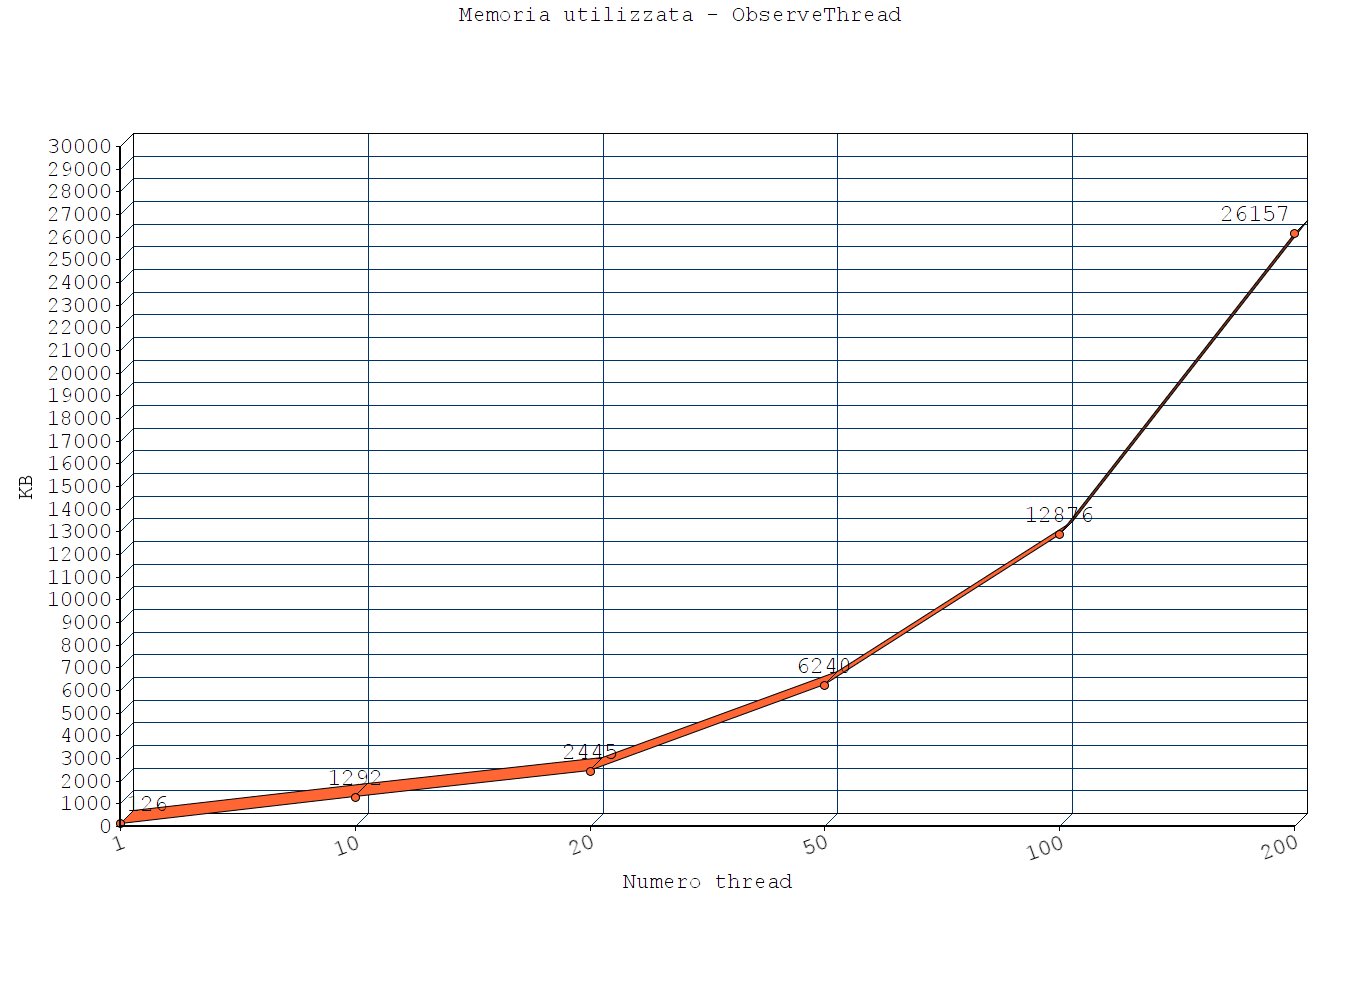
\includegraphics[width=\textwidth]{immagini/observe.png}
\caption{\textit{La crescita di memoria per i thread {\tt Observe}}}
\end{figure}
\begin{figure}[p]
\centering
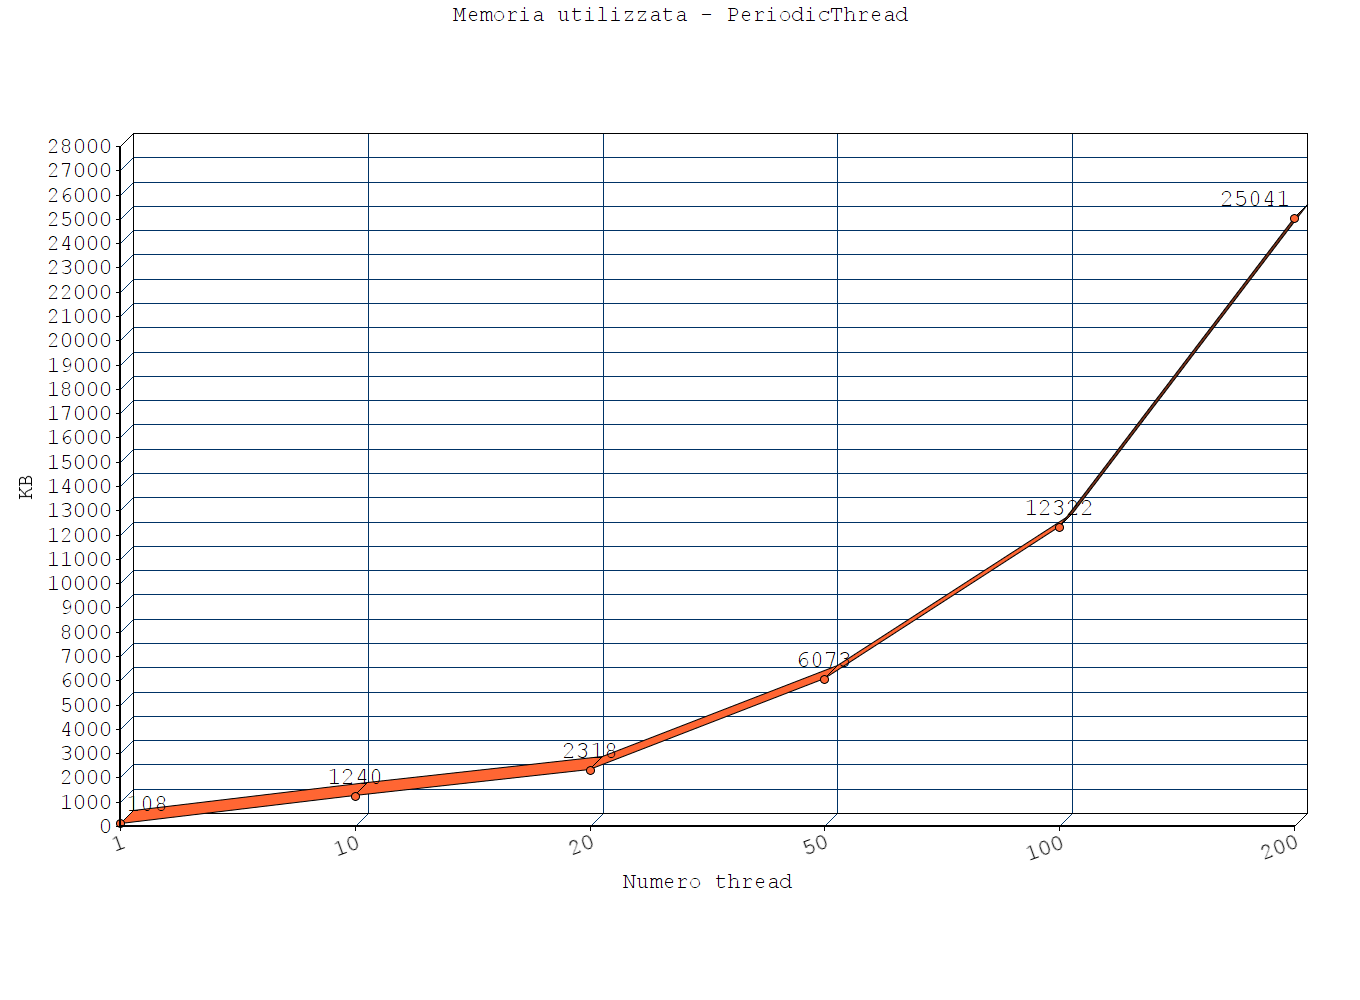
\includegraphics[width=\textwidth]{immagini/periodic.png}
\caption{\textit{La crescita di memoria per i thread {\tt Periodic}}}
\end{figure}

\vspace{1.0cm}
Come è possibile notare la crescita di richiesta di memoria è abbastanza lineare, permettendo al sistema di essere sufficientemente scalabile e relativamente leggero. La leggerezza del sistema potrebbe permettere di installare il sistema di monitoraggio su qualunque dispositivo che sia in grado di sostenere la Java Virtual Machine, come per esempio il noto Raspberry Pi, garantendo la possibilità di utilizzo non solo su sistemi distribuiti ad alte prestazioni ma anche in ambienti più ristretti come un'abitazione o una piccola azienda.
\\\\È stata testata la portabilità del sistema su sistemi operativi differenti (Windows e Linux) con successo, riscontrando una differenza prestazionale quasi nulla tra i due sistemi. La portabilità è un fattore importante in quanto il sistema server potrebbe essere potenzialmente configurato e installato su sistemi e architetture differenti per rispondere ad esigenze d'uso differenti.
\\Il sistema di monitoraggio è predisposto per poter funzionare con interfacce differenti da quella Web utilizzata, essendo necessario semplicemente effettuare delle chiamate RPC alla cloud, e può quindi essere attivato, per esempio da una applicazione per smartphone oppure in automatico da un altro server.
\\\\Il sistema è anche interoperabile, in quanto è in grado di monitorare una qualunque risorsa che sia in grado di comunicare tramite protocollo CoAP che, essendo estremamente leggero e versatile, è adatto a funzionare sulla stragrande maggioranza degli smart objects. È stata inoltre testata la possibilità di monitorare sia reti basate su protocollo IPv4 che IPv6 che misto, con grande successo, garantendo al sistema di essere in grado di prelevare dati da reti di diversa natura.

\section{Scenari d'uso}
I possibili scenari d'utilizzo del sistema di monitoraggio sono molteplici: si potrebbe immaginare, per esempio, un sistema distribuito sul quale la cloud è installata su di un server o magari un cluster in cloud, il DBMS è installato su di un altro server e l'interfaccia Web su un terzo server. Le reti da monitorare potrebbero essere, per esempio, reti di sensori che rilevano l'occupazione dei parcheggi pubblici in una città e l'utente, tramite interfaccia Web o tramite app per smartphone, potrebbe monitorare i parcheggi sotto casa per sapere in tempo reale quando uno diventa libero, utilizzando un connettore che lo avvisa via email.
\\Oppure cloud, DBMS e interfaccia potrebbero essere installati su di un PC in casa che monitora lo stato di alcuni sensori, come sensori di temperatura e umidità, sensori di movimento, di rilevamento gas ecc... per aggiornare un profilo Twitter pubblico e mantenere lo storico delle temperature nelle varie stanze ed essere allertati quando viene rilevata una fuga di gas.
\\\\O ancora, il sistema cloud potrebbe essere di dominio pubblico e un'azienda potrebbe creare la propria interfaccia per monitorare lo stato di alcuni sensori posti all'interno dell'azienda stessa, per avere una stima della produzione giornaliera, per esempio, o per stimare l'utilizzo di corrente. I dati potrebbero essere inviati tramite un connettore customizzato ad un database interno all'azienda per essere successivamente analizzati e perfezionare così l'andamento dei processi aziendali.
\\\\Le possibilità offerte sono tantissime e gli scenari profilabili altrettanti. È necessario solamente avere a disposizione una rete di sensori che siano in grado di comunicare tramite protocollo CoAP.

\section{Possibili sviluppi futuri}
Alcuni possibili sviluppi futuri potrebbero rendere il sistema cloud ancora più interessante. Delle possibili espansioni potrebbero essere:
\begin{itemize}
\item L'aggiunta di nuovi connettori, oltre al già presente Twitter, come Facebook, Telegram, email, pubblicazione di pagine HTML ecc...
\item La possibilità per la cloud di effettuare automaticamente la discovery di nuove risorse nella rete e notificare la presenza all'utente tramite connettori oppure creare automaticamente un'azione di monitoraggio per le nuove risorse.
\item La creazione di una vera e propria API per l'accesso alla cloud, costruendo uno strato di astrazione per le chiamate XML-RPC, rendendo così disponibili le operazioni di creazione e cancellazione di azioni anche da interfacce esterne senza necessariamente effettuare chiamate RPC.
\item L'aggiunta di nuove chiamate RPC alla cloud, con la possibilità di ottenere il livello di carico del sistema in tempo reale. Sarebbe possibile effettuare questa espansione sfruttando lo stesso paradigma di monitoraggio, rendendo la cloud stessa una risorsa, uno smart object che notifica in tempo reale a sè stesso, e quindi all'utente che ne ha richiesto il monitoraggio, il proprio stato.
\item L'inclusione di altri protocolli IoT, come MQTT, per rendere possibile il monitoraggio sul maggior numero possibile di smart objects e ampliare ulteriormente l'area di operabilità del sistema.
\end{itemize}

\pagestyle{fancy}
\renewcommand{\chaptermark}[1]{\markboth{#1}{}}
\renewcommand{\sectionmark}[1]{\markright{#1}{}}
\fancyhf{}
\rhead{\rightmark}
\cfoot{\thepage}

\phantomsection
\addcontentsline{toc}{chapter}{Conclusioni}
\chapter*{Conclusioni\markboth{}{Conclusioni}}
%\pagestyle{fancy}
\renewcommand{\chaptermark}[1]{\markboth{#1}{}}
\renewcommand{\sectionmark}[1]{\markright{#1}{}}
\fancyhf{}
\rhead{\rightmark}
\cfoot{\thepage}

\phantomsection
\addcontentsline{toc}{chapter}{Ringraziamenti}
\chapter*{Ringraziamenti\markboth{}{Ringraziamenti}}

Il primo ringraziamento, sentito quanto sincero, va alla mia famiglia:
ai miei genitori Marco e Rita, e ai miei fratelli Matteo ed Emanuele;
sostegno sempre sicuro, anche nei momenti più complicati.
Un grazie speciale a Federica, compagna incrollabile, sempre pronta a
supportarmi (e sopportarmi).

Ringrazio poi tutti i docenti del Corso di Laurea di Informatica, in
particolare il mio relatore Enea Zaffanella, capace di trasmettere
conoscenza ed entusiasmo, sempre disponibile al dialogo e al confronto.

Vorrei citare anche i professori del Liceo Classico Romagnosi di Parma,
in particolare Michele Abbati, Patrizia Aiello, Giovanni Brunazzi,
Maurizio Olivieri e Monica Silingardi.

Un ringraziamento a Sebastian, Dottore dentro e fuori; a Paolo, con i
suoi aneddoti sportivi; a Federico e i suoi cellulari; a Maxim,
compare di caffè; a Jacopo e le sue giocate; a Luca e i suoi cavi, a
Francesco con la sua password, ad Alessio e le sue idee; a Daniela, con
i suoi modi di dire, e ad Eleonora e le discussioni letterarie.

Infine, un ringraziamento a tutti gli altri che mi hano supportato: a
Luca, da Londra, che mi ha fatto scoprire l'Informatica (e altre brutte
cose da nerd); a Pietro, Francesco e Michele, compagni di bevute
insostituibili; a Massimiliano, Davide e Filippo, Master impareggiabili;
ad Andrea e al suo cacciavite.

A dodo e degustazioni, a giochi di ruolo e videogiochi, a grigliate e
serie TV; grazie di tutto, a tutti.

% Bibliografia.
\cleardoublepage
\phantomsection
\addcontentsline{toc}{chapter}{Riferimenti bibliografici}
\begin{thebibliography}{}

\bibitem{atmel} Atmel Corporation Blog\\
  \emph{A look back at the history of the Internet of Things} \\
  \footnotesize \texttt{\url{http://blog.atmel.com/2015/04/09/a-look-back-at-the-history-of-the-internet-of-things/}} \\
  
\bibitem{active-badge} Roy Want, Andy Hopper, Veronica Falcão, Jonathan Gibbons\\
  \emph{The Active Badge Location System} \\
  \footnotesize \texttt{\url{http://alumni.media.mit.edu/~dmerrill/badge/Want92_ActiveBadge.pdf}} \\
  
\bibitem{internet-toaster} Living Internet\\
  \emph{The Internet Toaster} \\
  \footnotesize \texttt{\url{http://www.livinginternet.com/i/ia_myths_toast.htm}} \\
  
\bibitem{coffee-pot} Daniel Gordon\\
  \emph{The Trojan Room Coffee Pot} \\
  \footnotesize \texttt{\url{http://www.cl.cam.ac.uk/coffee/coffee.html}} \\
  
\bibitem{mqtt-faq} MQTT\\
  \emph{FAQ} \\
  \footnotesize \texttt{\url{http://mqtt.org/faq}} \\
  
\bibitem{itu-iot} International Telecommunication Union\\
  \emph{ITU Internet Reports 2005: The Internet of Things} \\
  \footnotesize \texttt{\url{http://www.itu.int/osg/spu/publications/internetofthings/}} \\
  
\bibitem{linky} ERDF\\
  \emph{Smart Meters, ERDF continue deploying Linky} \\
  \footnotesize \texttt{\url{http://www.erdf.fr/sites/default/files/documentation/DP_ERDF_210610_1_EN.pdf}} \\
  
\bibitem{its} United States Department of Transportation\\
  \emph{Intelligent Transportation Systems Joint Program Office} \\
  \footnotesize \texttt{\url{http://www.its.dot.gov/connected_vehicle/connected_vehicle_tech.htm}} \\
  
\bibitem{mantova-pc} Mantova Phygital City Website\\
  \emph{Mantova Phygital City} \\
  \footnotesize \texttt{\url{http://www.mantovaphygitalcity.it}} \\
  
\bibitem{varese-sc} Varese Smart City Website\\
  \emph{Il progetto Varese Smart City} \\
  \footnotesize \texttt{\url{http://www.varesesmartcity.com/ita/varese/1-Il-Progetto-Varese-SmartCity.aspx}} \\
  
\bibitem{alcatel} Alcatel-Lucent Techzine\\
  \emph{How smart cities can improve our lives} \\
  \footnotesize \texttt{\url{https://techzine.alcatel-lucent.com/how-smart-cities-can-improve-our-lives}} \\
  
\bibitem{roland-berger} Roland Berger Press Room\\
  \emph{INDUSTRY 4.0: THE DIGITAL WORLD PROVIDES NEW OPPORTUNITIES FOR EUROPEAN INDUSTRY TO MOVE INTO A NEW ERA
} \\
  \footnotesize \texttt{\url{http://www.rolandberger.com/press_releases/Industry_4_0_opportunities_for_European_industry.html}} \\
  
\bibitem{802-15-4} Dr. José A. Gutierrez\\
  \emph{Enabling Pervasive Wireless Sensor Networs} \\
  \footnotesize \texttt{\url{http://www.cs.berkeley.edu/~prabal/teaching/cs294-11-f05/slides/day21.pdf}} \\
  
\bibitem{survey} Luigi Atzori, Antonio Iera, Giacomo Morabito\\
  \emph{The Internet of Things: A survey} \\
  \footnotesize \texttt{Computer Networks Journal number 54 (2010)} \\
  
\end{thebibliography}


\end{document}
